%% This template is based on the sample-acmtog template from overleaf.

%% The first command in your LaTeX source must be the \documentclass command.
\documentclass[acmtog, nonacm]{acmart}

%% \BibTeX command to typeset BibTeX logo in the docs
\AtBeginDocument{%
  \providecommand\BibTeX{{%
    \normalfont B\kern-0.5em{\scshape i\kern-0.25em b}\kern-0.8em\TeX}}}

\setcopyright{none}

\citestyle{acmauthoryear}

\usepackage{tikzducks}
\usepackage{microtype}
\emergencystretch 5em
%%
%% end of the preamble, start of the body of the document source.
\begin{document}

\title{Steer Engine: A Performance-Focused ECS Engine for Vehicular Action Games}
\subtitle{Group Report for COMP 5531M}

\author{Sicheng Chen}
\authornote{Sharing first authorship}
\email{sc22sg@leeds.ac.uk}

\author{Samuil Georgiev}
\authornotemark[1]
\email{sc22sg@leeds.ac.uk}

\author{Qidan Guo}
\authornotemark[1]
\email{sc22sg@leeds.ac.uk}

\author{Harry Li}
\authornotemark[1]
\email{sc22sg@leeds.ac.uk}

\author{Chenghao Zhu}
\authornotemark[1]
\email{sc22sg@leeds.ac.uk}

\author{Rafael Kuffner dos Anjos}
\authornote{Supervisor}
\email{r.kuffnerdosanjos@leeds.ac.uk}

\affiliation{%
  \institution{University of Leeds}
  \streetaddress{Woodhouse}
  \city{Leeds}
  \state{West Yorkshire}
  \country{United Kingdom}
  \postcode{LS2 9BW}
}

\begin{abstract}
  \textcolor{blue}{This section here is the abstract, which is a summary of your work in no more than \textbf{150 words}.}
  As game engines evolve into monolithic toolsets, they introduce unnecessary overhead for genre-specific applications. We present our custom, performance-focused game engine built entirely in C++, leveraging Vulkan for rendering, Flecs for Entity-Component-System (ECS) data locality, and Jolt Physics for deterministic vehicular simulation. By utilizing a pure ECS paradigm, we achieve high-performance entity management with negligible CPU bottlenecks. To demonstrate the engine, we developed a fast-paced bicycle action game requiring high-speed collision resolution and physics-driven mechanics. Our engine development focused on a robust core loop, hardware-accelerated Vulkan rendering, tuned rigid-body dynamics, and comprehensive tooling. The resulting Steer Engine reliably powers the vehicular demo, validating that targeted architectures can outperform generalized engines for specific domains.
\end{abstract}

\begin{CCSXML}
<ccs2012>
   <concept>
       <concept_id>10003752.10003809.10010052</concept_id>
       <concept_desc>Theory of computation~Parameterized complexity and exact algorithms</concept_desc>
       <concept_significance>100</concept_significance>
       </concept>
   <concept>
       <concept_id>10010583.10010750</concept_id>
       <concept_desc>Hardware~Robustness</concept_desc>
       <concept_significance>300</concept_significance>
       </concept>
   <concept>
       <concept_id>10010147.10010371.10010396.10010401</concept_id>
       <concept_desc>Computing methodologies~Volumetric models</concept_desc>
       <concept_significance>500</concept_significance>
       </concept>
 </ccs2012>
\end{CCSXML}

\ccsdesc[100]{Theory of computation~Parameterized complexity and exact algorithms}
\ccsdesc[300]{Hardware~Robustness}
\ccsdesc[500]{Computing methodologies~Volumetric models}

\keywords{Game Engine, Vulkan, ECS, Flecs, Jolt Physics, Vehicular Simulation}

\maketitle

\section{Introduction}
\textcolor{blue}{The introduction of your report must give the reader some context, motivation for choosing this as a project, describing what you did, and giving a sneak peak of your results.
This works as a way of getting someone to read the rest of the paper, almost like a pitch.
The whole report should be no more than 12 pages, references and figures included. 
4 Pages are reserved for project management on the appendix. }

As game engines have evolved into monolithic toolsets (e.g., Unreal Engine, Unity), they inherently provide generalized architectures to cater to a massive variety of genres. While convenient, this generalization introduces unnecessary overhead, convoluted component hierarchies, and rigidity that can hinder performance-critical, genre-specific applications. We present our custom, performance-focused game engine built entirely in C++, leveraging the explicit graphics control of Vulkan, the rigorous data-locality of Flecs (an Entity-Component-System), and the deterministic physical simulation capabilities of Jolt Physics.

Our primary goal was to construct a scalable architecture specialized in vehicular mechanics and expansive environments, while maintaining the flexibility to incorporate advanced stylisation and rendering features. By abandoning deep inheritance trees in favor of a pure ECS paradigm, we achieve high-performance entity management, capable of handling complex level assemblies with negligible CPU bottlenecks.

To demonstrate the engine's capabilities, we developed a fast-paced bicycle action game. In this demo, the player controls a bicycle traversing a custom level geometry, aiming to collect scattered boosters. Once all boosters are collected, the player acquires enhanced speed and jumps off a designated ramp to clear the level's enclosing walls. This action effectively completes the stage and seamlessly transitions the player to the next.

Our engine development focuses on four main pillars:
\begin{enumerate}
    \item \textbf{Core Architecture}: An optimized, ECS-driven game loop handling engine life-cycle, event dispatching, and scene management.
    \item \textbf{Physically Based Rendering (PBR)}: A Vulkan-based backend providing hardware-accelerated Shadow Mapping, Alpha Masking, Post-Processing, and debug visualisations.
    \item \textbf{Rigid Body Dynamics}: Integration of Jolt Physics with a specialized Vehicle Constraint system for robust, tunable bicycle control.
    \item \textbf{Tooling \& Scalability}: ImGui integration, input action mapping, and level assembly pipelines.
\end{enumerate}

While early prototypes lacked full audiovisual polish, the core engine loop now integrates a comprehensive Audio System powered by miniaudio, a Particle System for visual effects, and a Skeletal Animation System featuring Inverse Kinematics. This robust foundation reliably powers a fully playable, physics-driven vehicular demo, demonstrating scalable performance.

\section{Background Research}
\label{sec:background}
\textcolor{blue}{Your background research should include a detailed review of known industry/academic work, and how they relate to what you want to do.
It should not be simply a list of papers/methods with a short description about them.
Instead, it should put them in context, establishing relationships, differences, highlights, limitations, and ultimately relating them to your proposed work. 
You should not need to explain concepts that are already known by the reader. 
The readers for your project will be academic staff at this university, so while there are some concepts that are important to introduce, you do not need to explain what a computer is. 
Remember the old saying: Don't preach to the choir.
Overall, this section should allow readers to understand what people in this field have been doing.}

\subsection{Game Engines and Architectural Patterns: OOP vs. ECS}
Modern game development largely depends on foundational software frameworks known as game engines. Historically, engines have relied heavily on deep inheritance structures and Object-Oriented Programming (OOP) to manage entities, a pattern extensively documented by Jason Gregory in his seminal work \textit{Game Engine Architecture} \cite{GameEngineArch}. For example, a game entity might inherit from \texttt{GameObject}, which inherits from \texttt{Transformable}, which inherits from \texttt{BaseNode}.

\textbf{Drawbacks of OOP Engines}: While OOP provides intuitive hierarchical modeling, deep inheritance often leads to the "Deadly Diamond of Death" and rigid class structures that are difficult to refactor. More critically, OOP engines suffer from poor memory data-locality. Objects are scattered across the heap, causing frequent CPU cache misses when iterating over large numbers of entities, which severely degrades performance in environments crowded with interactive elements. This limitation is heavily criticized in Richard Fabian's \textit{Data-Oriented Design} \cite{DataOrientedDesign}, which advocates for memory contiguity.

\textbf{Advantages of ECS (Flecs)}: To overcome these limitations, our engine embraces the Entity-Component-System (ECS) pattern, specifically utilizing Sander Mertens' \textit{Flecs} \cite{Flecs}, similar to the robust ECS implementation seen in Blizzard's \textit{Overwatch} gameplay architecture \cite{OverwatchECS}. In ECS, entities are merely lightweight integer IDs, components are plain-old-data (POD) structs, and systems contain the logic that iterates over specific component combinations. The primary importance of ECS is its excellent CPU cache locality. Components of the same type are stored contiguously in memory arrays, enabling highly efficient batch processing. This architecture fundamentally justified our choice of Flecs, allowing us to manage massive amounts of dynamic entities (e.g., thousands of custom level particles and instanced geometries) without traditional CPU bottlenecks.

\subsection{Real-Time Graphics: Vulkan vs. OpenGL/DirectX}
Real-time rendering APIs serve as the bridge between engine logic and the GPU. Legacy APIs like OpenGL and earlier versions of DirectX (DX11) manage a significant amount of state implicitly behind the scenes.

\textbf{Drawbacks of Legacy APIs (OpenGL/DX11)}: While easier to learn, OpenGL suffers from unpredictable driver overhead and opaque thread management. The driver implicitly handles memory allocation and synchronization, taking away optimization opportunities from the developer. This often results in CPU-bound rendering bottlenecks, a well-known limitation of OpenGL as described in the \textit{OpenGL SuperBible} \cite{OpenGLSuperBible}.

\textbf{Advantages of Explicit APIs (Vulkan)}: The industry has shifted toward explicit APIs like Vulkan and DirectX 12. Vulkan gives developers granular control over GPU memory, explicit synchronization barriers, and multi-threaded command buffer dispatching, a paradigm shift popularized by high-performance engines like idTech 6 in \textit{DOOM Eternal} \cite{DoomEternal, DoomVulkan}. Despite the steep learning curve and highly verbose setup required, Vulkan was chosen for our engine because it completely eliminates unpredictable driver overhead. It allows our custom \texttt{RenderSystem} to meticulously define sub-passes, handle explicit image layout transitions, and construct precise rendering pipelines. These capabilities are essential for implementing performant Physically Based Rendering (PBR), hardware Percentage-Closer Filtering (PCF), and dynamic shadow mapping without sacrificing frame rates.

\subsection{Vehicular Physics: Jolt vs. PhysX and Bullet}
Simulating vehicular dynamics in real-time requires a robust physics solver capable of handling suspension, wheel friction, and high-speed collision detection without erratic jittering.

\textbf{Drawbacks of Generalised Physics Engines (PhysX/Bullet)}: NVIDIA's PhysX and the Bullet physics engine are the traditional industry standards. PhysX provides extensive features including soft bodies, fluid dynamics, and cloth simulation, as detailed in the NVIDIA PhysX SDK \cite{PhysX} and seen in titles like \textit{Cyberpunk 2077} \cite{CyberpunkVulkan}. However, this generalization introduces significant overhead. Bullet, while open-source and modular, can sometimes struggle with multithreaded scalability and deterministic rigid-body resting states under heavy loads, an issue sometimes encountered with the open-source Bullet Physics library \cite{BulletPhysics}.

\textbf{Advantages of Jolt Physics}: Jolt Physics \cite{JoltPhysics} has recently emerged as a high-performance alternative explicitly designed to prioritize speed, deterministic rigid-body simulation, and multithreaded scalability, as engineered by Jorrit Rouwe for \textit{Horizon Forbidden West} \cite{JoltHorizon, HorizonFW}. Jolt deliberately omits soft-body and fluid simulations to maintain a lightweight core. For our project, the deciding factor was Jolt's built-in \texttt{VehicleConstraint} system. It provides a highly configurable interface for raycast-based wheel suspension, damping, and custom friction simulation, heavily inspired by arcade-racer mechanics seen in commercial titles like \textit{Need for Speed Unbound} \cite{NFSUnbound, NFSUnboundTech} and \textit{Mario Kart 8} \cite{MarioKart8}. This explicitly tailored rigid-body focus made Jolt the ideal candidate to handle the high-speed ramps, collision shapes, and dynamic torque requirements of our bicycle mechanics without the bloat of an overarching generalised physics system.

\section{Methodology: Engine Architecture \& Implementation}

\begin{figure}[h]
  \centering
  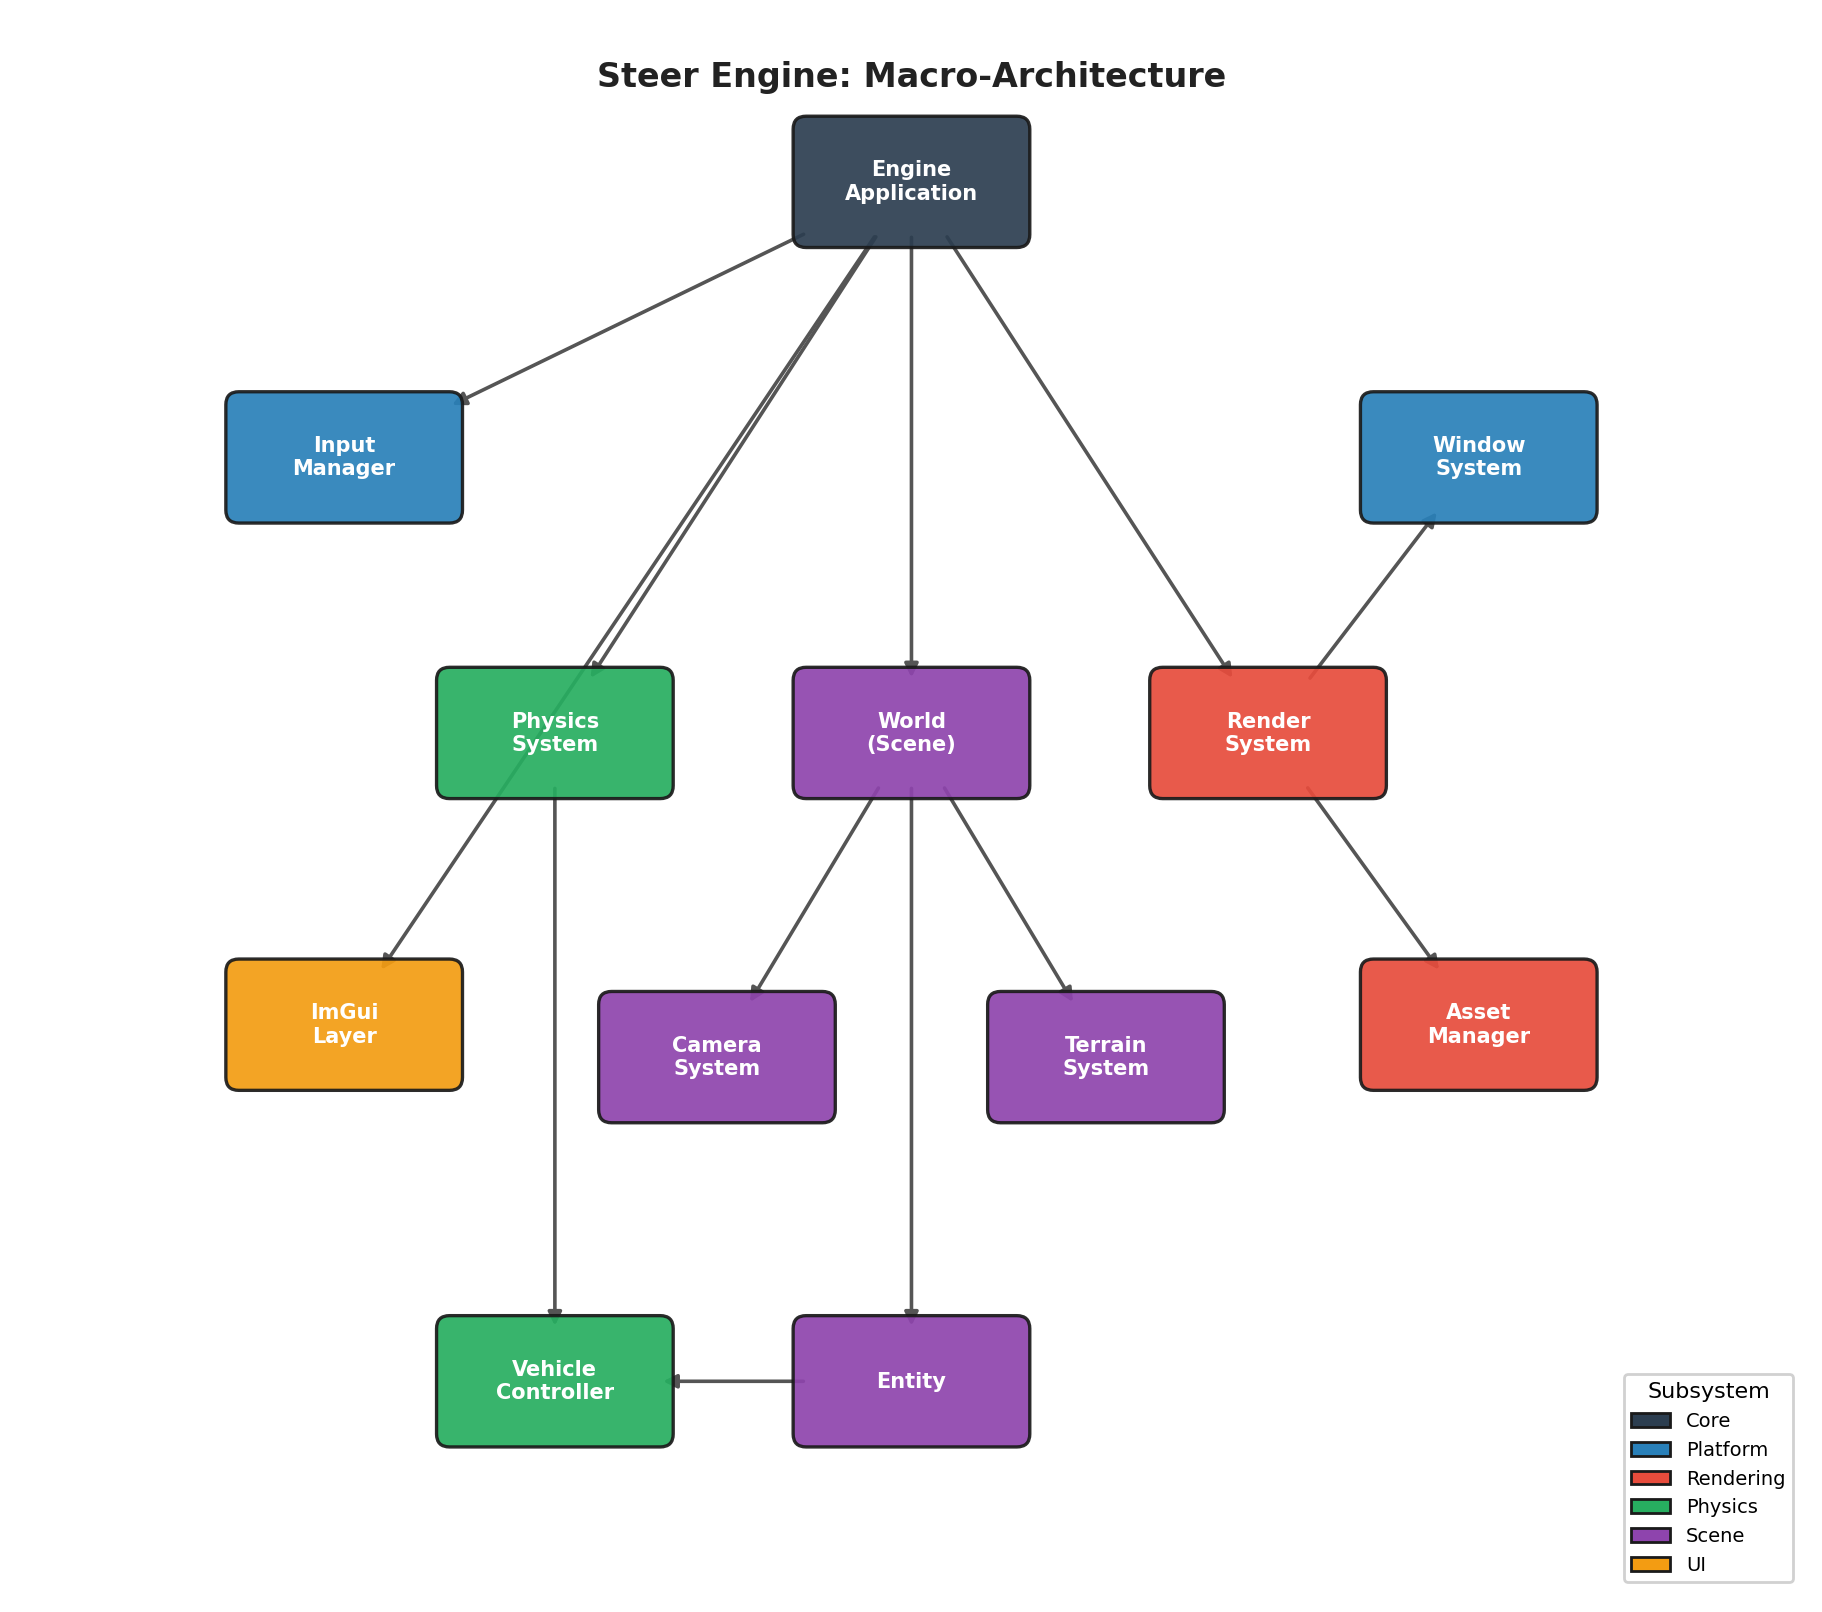
\includegraphics[width=\linewidth]{simplified_architecture.png}
  \caption{\textbf{Simplified Engine Macro-Architecture.} Directed edges represent ownership or primary data-flow relationships. The \texttt{EngineApplication} orchestrates five top-level subsystems; the \texttt{World} manages scene-graph entities, camera, and terrain; the \texttt{RenderSystem} owns the Vulkan backend and asset pipeline.}
  \label{fig:architecture}
\end{figure}

The engine's macro-architecture, illustrated in Figure~\ref{fig:architecture}, is designed around a decoupled, data-driven methodology that isolates the main loop, scene management, physics simulation, and rendering pipelines into distinct subsystems. The core structural interactions can be summarised as follows:

\begin{itemize}
    \item \textbf{EngineApplication}: Acts as the overarching controller. It owns and coordinates the primary subsystems: \texttt{InputManager}, \texttt{PhysicsSystem}, \texttt{RenderSystem}, the \texttt{ImGuiLayer}, and the active \texttt{World}.
    \item \textbf{World}: Functions as the scene manager, holding the \texttt{CameraSystem}, \texttt{TerrainSystem}, and a collection of \texttt{Entity} objects. It bridges gameplay logic and rendering by processing entities and exposing them via \texttt{GetRenderables()}.
    \item \textbf{Entity}: Represents an individual game object in the world. Instead of complex inheritance, entities act as containers for components like transforms, mesh references, and physics bodies.
    \item \textbf{RenderSystem}: Drives the Vulkan backend. It references the \texttt{WindowSystem} for surface management, retrieves geometry and textures via the \texttt{AssetManager}, and compiles frame commands for GPU submission.
    \item \textbf{PhysicsSystem}: Encapsulates the Jolt Physics engine. It owns the \texttt{VehicleController} and is strictly responsible for updating spatial data and handling collision constraints for entities that possess a \texttt{PhysicsBody}.
\end{itemize}

\subsection{Core System and ECS Integration (Flecs)}
The engine's lifecycle is governed by the \texttt{Application} class, which acts as the central orchestrator. It initializes the core subsystems: Windowing via GLFW \cite{GLFW}, Renderer, Input, Events, Physics, and the \texttt{SceneManager}.

The core logic revolves around \textbf{Flecs}, our chosen ECS backend. 

\textbf{Justification for Flecs}: In a high-speed vehicular game like our bicycle demo, the engine must constantly update the transforms of the player, environmental triggers (boosters), and potentially hundreds of dynamic particles without hitching. Flecs provides rigorous data locality by packing components into memory arrays based on entity archetypes. This allows systems to iterate through homogeneous blocks of memory, maximizing CPU cache hits. This decoupled architecture inherently separates data from logic, ensuring that gameplay code remains cleanly separated from rendering and physics integration.

\subsubsection{Core Component Structs}
To fully exploit Flecs' cache locality, our components are defined as tightly packed, plain-old-data (POD) C++ structs without virtual functions. This ensures they can be copied directly in contiguous memory. Some of our core components include:
\begin{verbatim}
struct LocalTransform { glm::mat4 matrix; };
struct WorldTransform { glm::mat4 matrix; };
struct MeshComponent  { uint32_t meshIndex; };
struct PhysicsBody    { uint32_t bodyID; };
struct EntityStatus   { bool should_render; bool has_physics; };
\end{verbatim}

Each component is a plain-old-data (POD) struct containing only scalar or fixed-size matrix fields. They use no virtual functions and require no heap allocations. For example, \texttt{LocalTransform} and \texttt{WorldTransform} each wrap a single $4 \times 4$ affine matrix, while \texttt{MeshComponent} and \texttt{MaterialComponent} store lightweight 32-bit indices into the engine's unified geometry and material registries. The \texttt{PhysicsBody} component holds a Jolt \texttt{BodyID} handle alongside a boolean flag indicating dynamic status, and the \texttt{RenderBatch} component records vertex offsets, index offsets, and index counts into the shared Vulkan device-local buffer.

\begin{figure}[h]
  \centering
  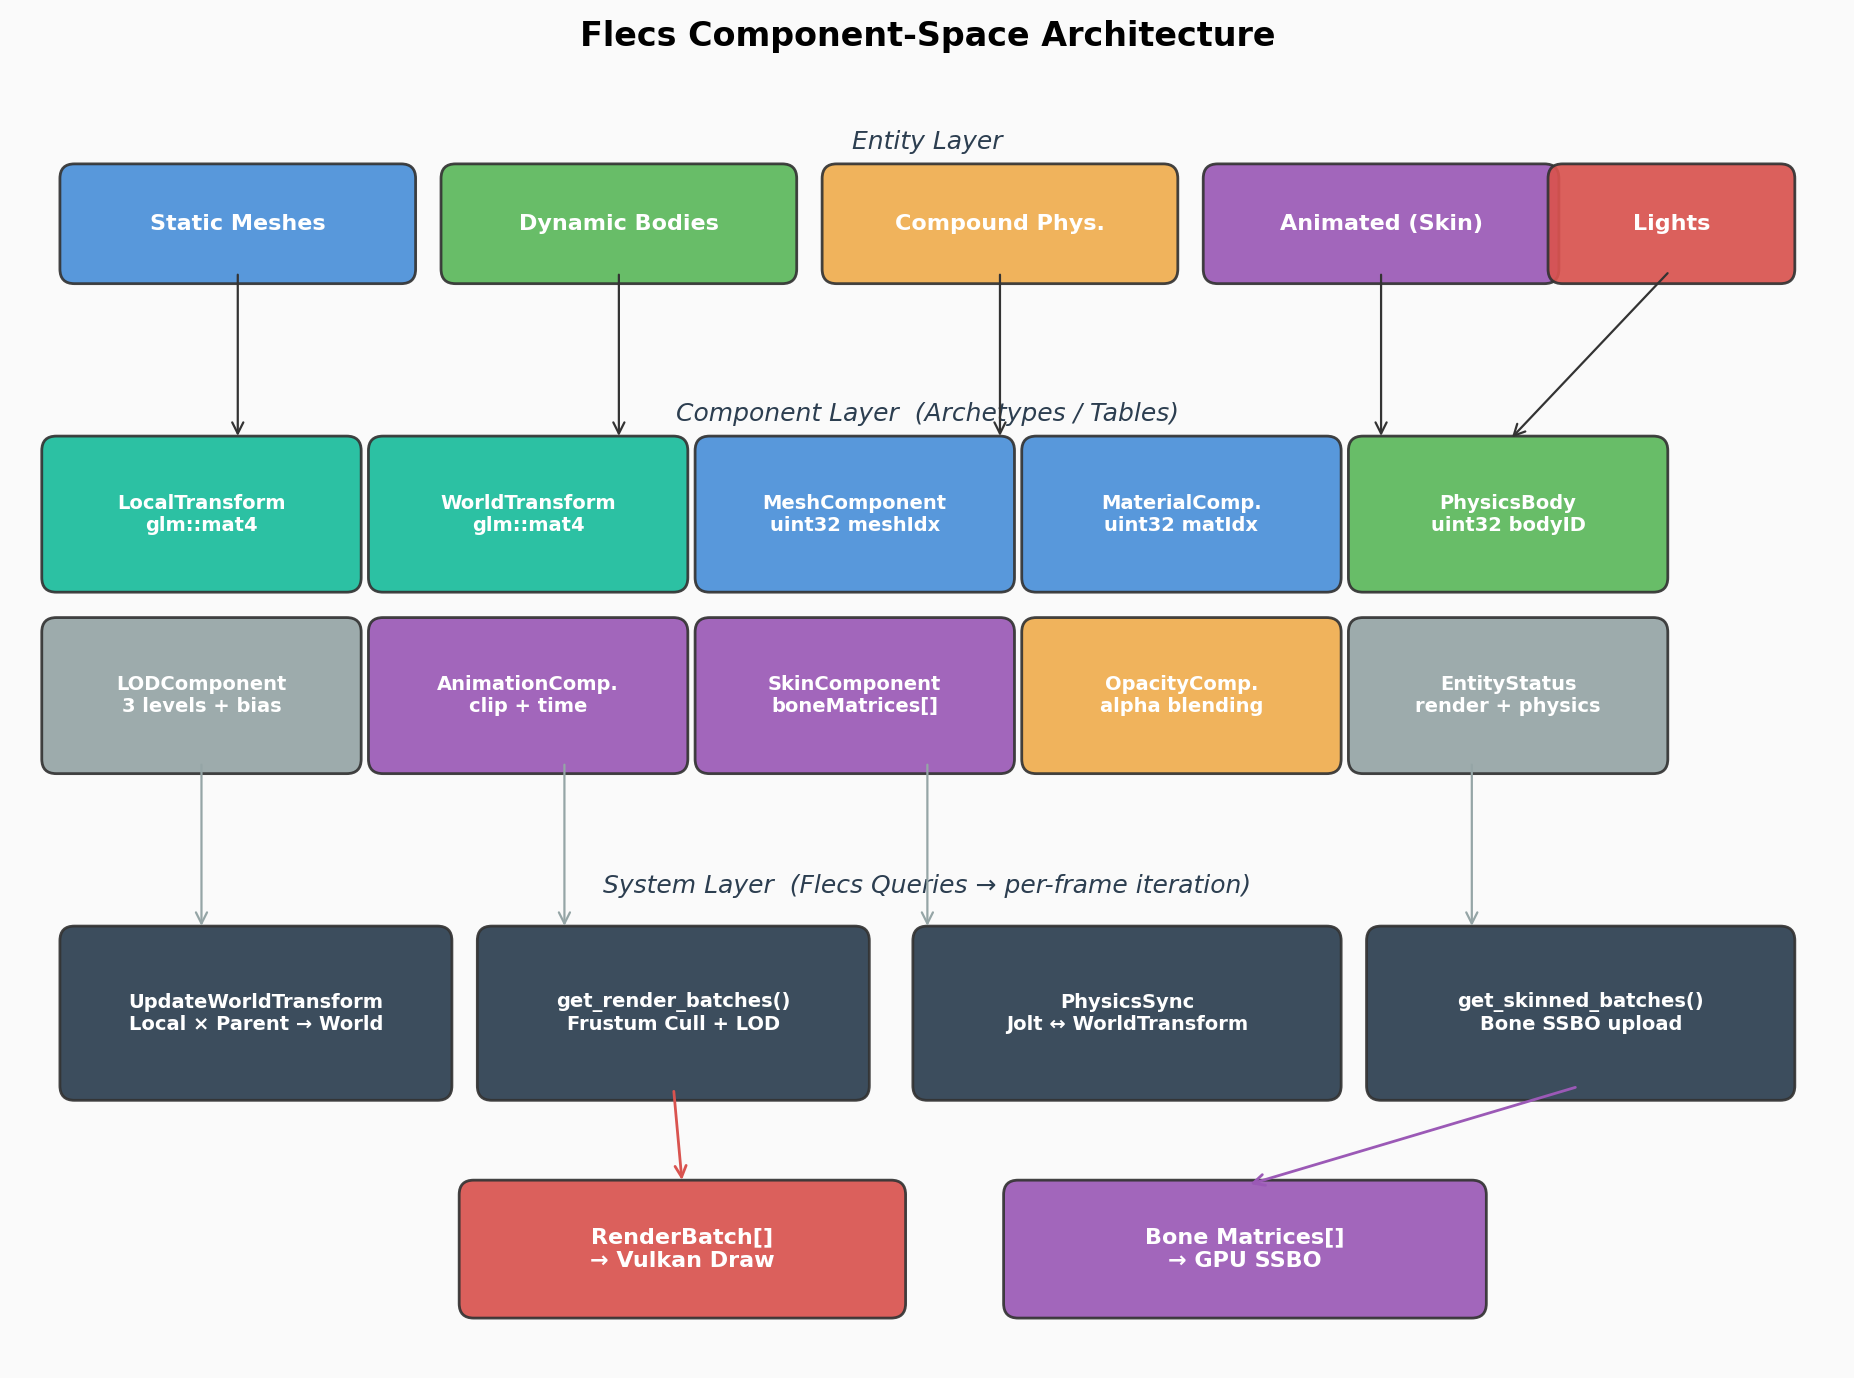
\includegraphics[width=\linewidth]{figures/flecs_component_space.png}
  \caption{\textbf{Flecs Component-Space Architecture.} Entities are grouped into archetypes based on their component signature. Components of identical type are packed contiguously, maximising CPU cache utilisation during system iteration. Arrows indicate the data flow from the \texttt{SceneManager} parse stage through archetype assignment to per-frame system queries.}
  \label{fig:flecs_archetype}
\end{figure}
These lightweight structs form the archetypes for our entities. For example, a static renderable obstacle consists of a \texttt{WorldTransform}, a \texttt{MeshComponent}, a \texttt{MaterialComponent}, and a \texttt{RenderBatch}. If it collides, it also contains a \texttt{PhysicsBody}.

\subsubsection{System Queries and Scheduling}
The power of Flecs lies in its ability to query entities that possess specific intersections of components. We define system queries to explicitly request access to arrays of components, which the ECS executes as batched arrays.

For instance, the \textit{UpdateWorldTransform} system requests mutable access to \texttt{WorldTransform} and read-only access to \texttt{LocalTransform}. For each matched entity, the system computes the world-space matrix $\mathbf{W}_e$ by composing the parent's cached world matrix with the entity's local matrix $\mathbf{L}_e$; root entities simply use their local matrix directly. Because Flecs iterates over contiguous archetype tables, this hierarchical propagation executes with minimal cache misses even for deeply nested scene graphs.

To guarantee deterministic engine behaviour and eliminate frame-tearing or physics-jitter, we explicitly defined the execution phases of our ECS pipeline. System scheduling was rigorously managed to ensure data mutations occur in a strictly linear pipeline:
\begin{enumerate}
    \item \textbf{Input Phase}: Parses hardware states and translates them into action events.
    \item \textbf{Pre-Physics Phase}: Applies gameplay logic (e.g., booster trigger deletions) and input torque to the \texttt{bikeController}.
    \item \textbf{Physics Tick}: Steps the Jolt simulation forward based on the fixed time-step.
    \item \textbf{Post-Physics Transform Sync}: A critical system that reads the simulated \texttt{JPH::BodyID} transforms and overwrites the \texttt{WorldTransform} components of dynamic entities. This explicitly occurs \textit{before} rendering.
    \item \textbf{Render Tick}: The \texttt{RenderSystem} iterates over the now accurately positioned \texttt{WorldTransform} and \texttt{RenderBatch} entities to populate the Vulkan command buffers.
\end{enumerate}

\subsubsection{Level Assembly and Parsing Pipeline}
The \texttt{SceneManager} is responsible for translating human-readable level layouts into optimized Flecs archetypes. Our level assembly pipeline is designed to parse incoming scene data configurations (such as simplified GLTF structures or custom JSON maps). 

When parsing a level file, the \texttt{SceneManager} iterates over the defined objects and immediately instantiates them as lightweight Flecs IDs. It then dynamically attaches components:
\begin{itemize}
    \item If the parsed node contains vertex data, the geometry is uploaded to the unified Vulkan staging buffer, and a \texttt{RenderBatch} and \texttt{MeshComponent} are assigned.
    \item If the node is flagged as a solid collider (like the jump ramp or the enclosing walls), the \texttt{SceneManager} automatically generates a static triangle mesh collider utilizing Jolt's shape generator and attaches the resulting \texttt{PhysicsBody} component to the entity.
    \item If the node is flagged as a booster, it receives a trigger volume component and an event-listener callback.
\end{itemize}

This data-driven pipeline guarantees that our levels can be authored in external 3D software and instantly digested into the tightly-packed, cache-friendly architecture the rest of the engine relies upon.

\subsection{Rendering System}
The Vulkan rendering pipeline forms the visual backbone of the engine. Based on the requirements from early development tasks, we transitioned from basic rasterisation to a modular, multi-pass architecture managed by the \texttt{RenderSystem}. 

\subsubsection{Vulkan Dynamic Rendering Setup}
To modernize the engine, our Vulkan backend utilizes the VK\_KHR\_dynamic\_rendering extension from the Vulkan 1.3 Specification \cite{VulkanSpec} to explicitly control state without the legacy rigid structures of \texttt{VkRenderPass} and \texttt{VkFramebuffer} objects. This significantly simplified our codebase when managing complex multi-pass rendering. 

Instead of pre-baking framebuffers, we begin rendering by populating \texttt{VkRenderingAttachmentInfo} structures per frame. This structure specifies the \texttt{imageView}, the \texttt{imageLayout} (e.g., \texttt{VK\_IMAGE\_LAYOUT\_COLOR\_ATTACHMENT\_OPTIMAL}), and the \texttt{loadOp}/\texttt{storeOp} for each attachment. We then bind these attachments to a \texttt{VkRenderingInfo} struct, which defines the render area and layer count. 

At the start of each frame, the renderer populates per-attachment descriptors specifying the target image view, the desired image layout (e.g., \texttt{COLOR\_ATTACHMENT\_OPTIMAL}), and the load/store operations. These descriptors are aggregated into a single rendering info structure that defines the render area, layer count, colour attachment array, and depth attachment reference. The command buffer then begins a dynamic rendering scope against these descriptors, eliminating the need for statically pre-baked framebuffer objects.

\begin{figure}[h]
  \centering
  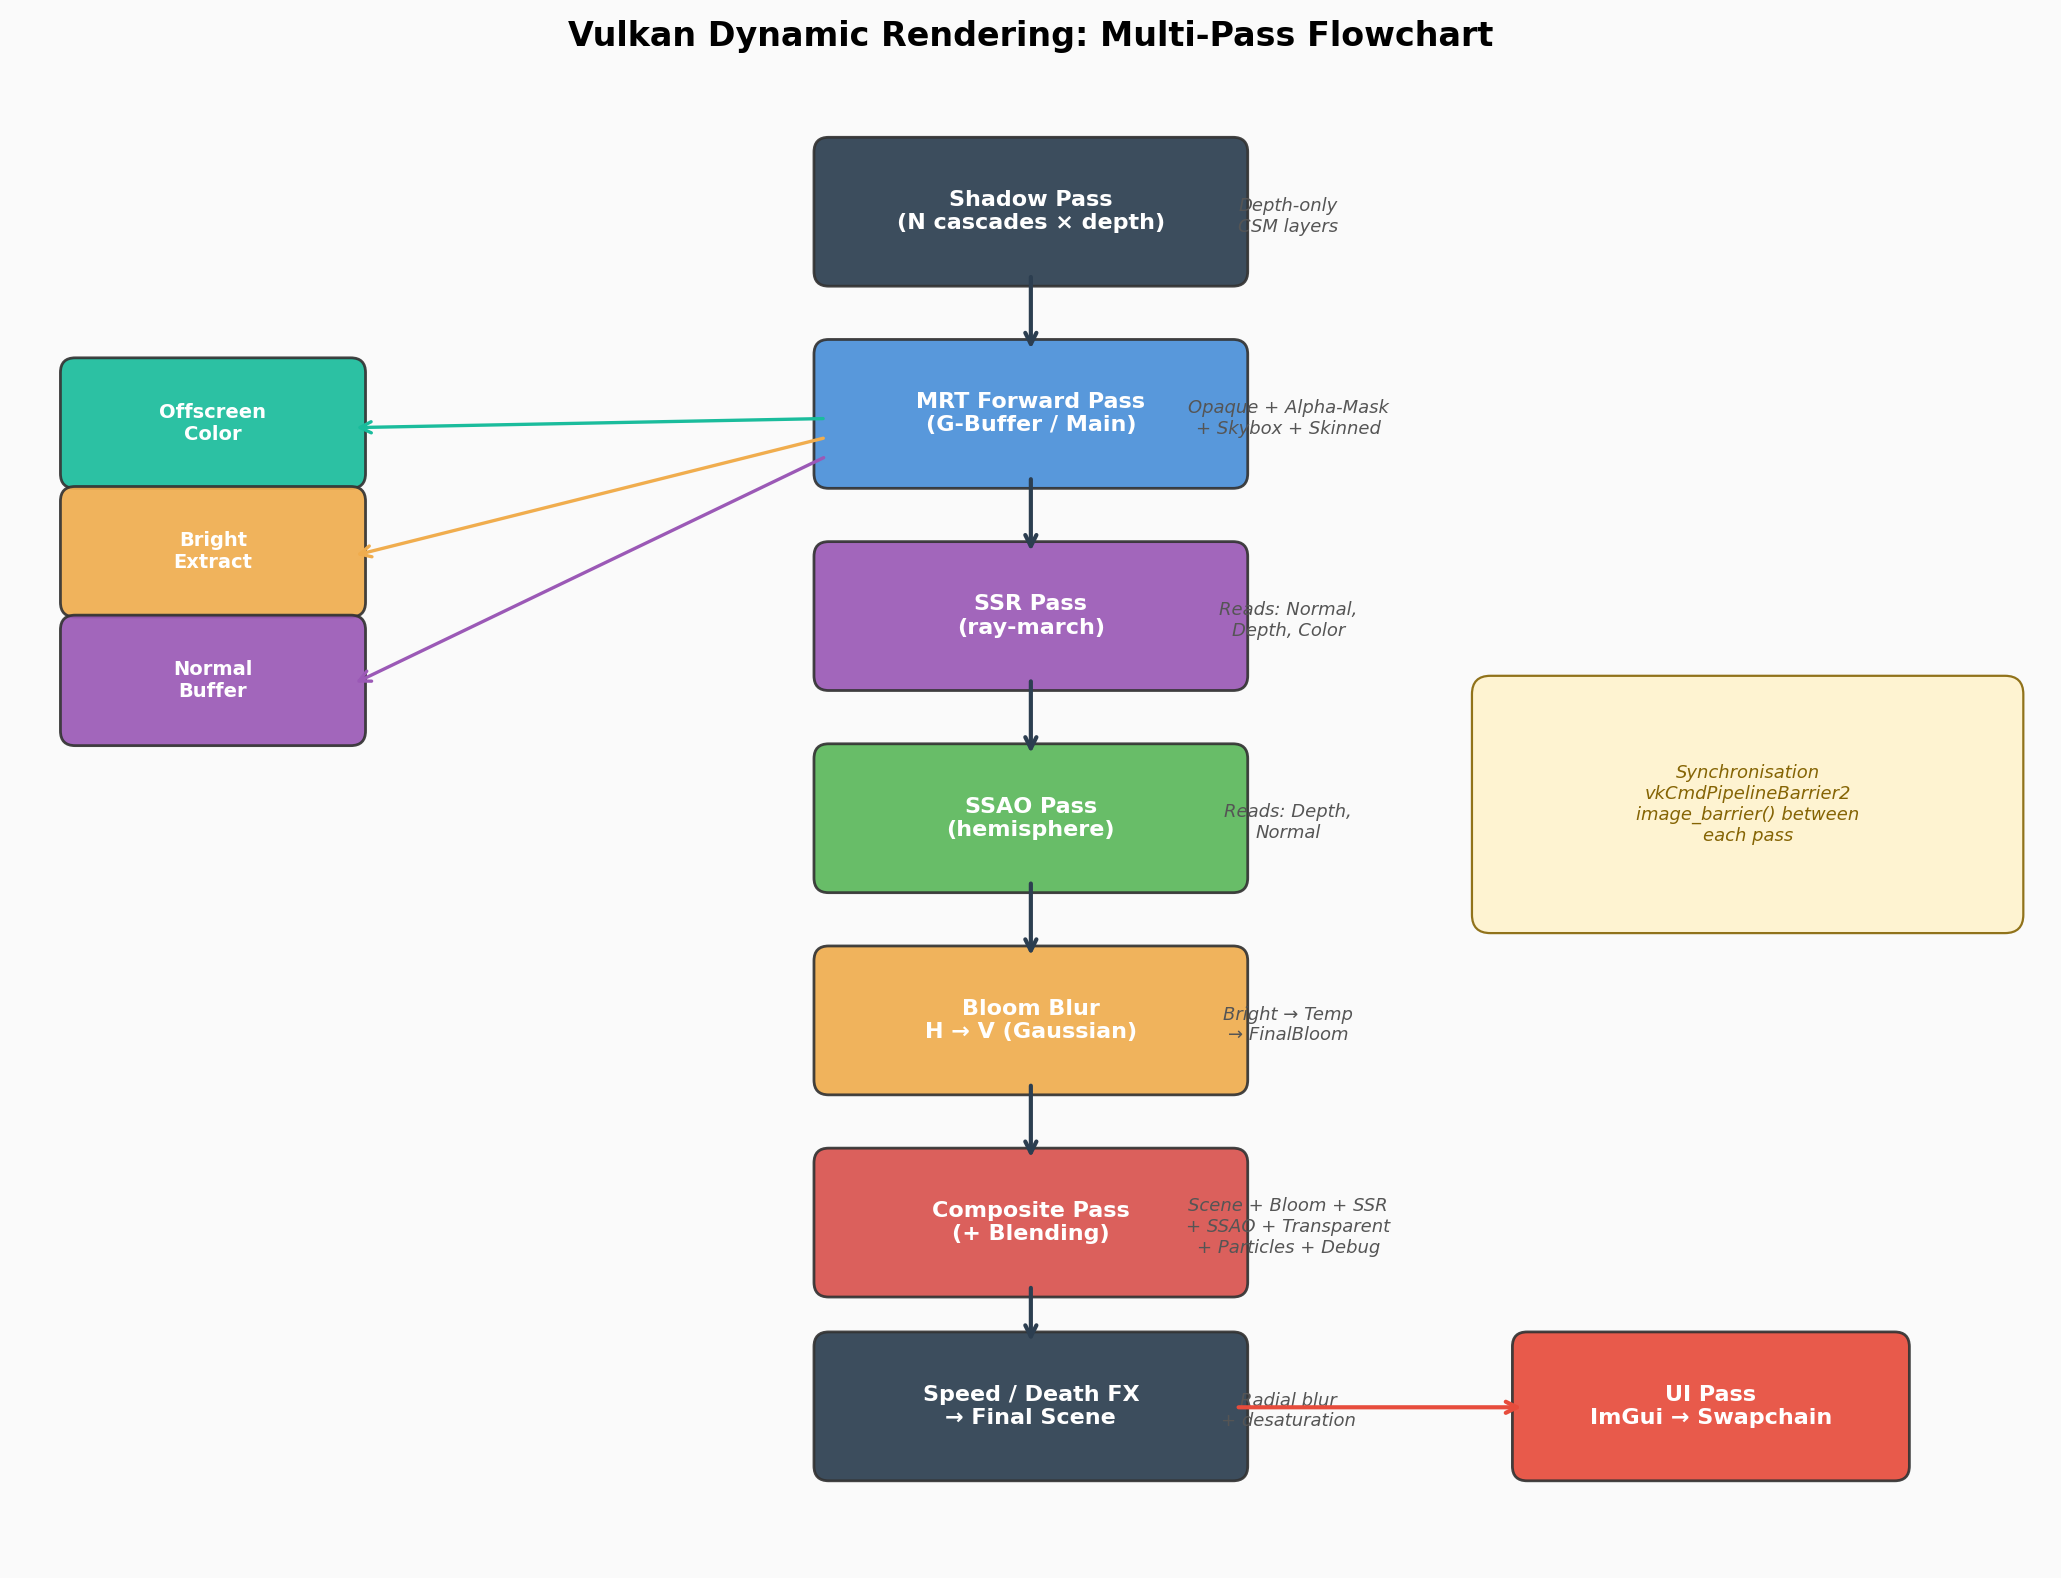
\includegraphics[width=\linewidth]{figures/render_pass_flowchart.png}
  \caption{\textbf{Render Pass Flowchart.} Data flow through the engine's multi-pass Vulkan pipeline. Each pass operates on explicit attachment descriptors; pipeline barriers enforce layout transitions and execution dependencies between the Shadow, Forward, Alpha-Mask, and Post-Processing stages.}
  \label{fig:render_flowchart}
\end{figure}

We rely heavily on explicit synchronization primitives. Before calling \texttt{vkCmdBeginRendering}, we insert pipeline barriers using \texttt{vkCmdPipelineBarrier} to explicitly transition image layouts (e.g., from \texttt{VK\_IMAGE\_LAYOUT\_UNDEFINED} to optimal attachment layouts) ensuring execution dependencies across our Shadow, Main Forward, and Post-Processing passes are strictly respected without GPU stalls.

\subsubsection{Data Management: UBOs and Descriptor Sets}
Supplying data to the shaders efficiently is critical for performance. We heavily utilize Uniform Buffer Objects (UBOs) to pass global scene parameters (View Matrix, Projection Matrix, Light Position, and Camera Position) to the vertex and fragment pipelines.

\textbf{std140 Memory Alignment}: A significant C++ implementation challenge was guaranteeing memory alignment between the CPU data structs (using GLM) and the Vulkan GLSL shader expectations. We strictly adhered to the \texttt{std140} layout rules. For instance, in our C++ struct, a \texttt{glm::vec3} (12 bytes) must be padded to 16 bytes. We explicitly added \texttt{alignas(16)} to our struct members to prevent subtle data corruption where Vulkan reads offset bytes:
\begin{verbatim}
struct alignas(16) ObjectPC {
    glm::mat4 transform;       // Offset 0,  Size 64
    glm::vec4 baseColorFactor; // Offset 64, Size 16
    glm::vec4 emissiveFactor;  // Offset 80, Size 16
    float metallicFactor;      // Offset 96, Size 4
    float roughnessFactor;     // Offset 100,Size 4
};
\end{verbatim}

Each field in the global uniform buffer is aligned to a 16-byte boundary in accordance with the \texttt{std140} layout specification. In particular, three-component vectors (12~bytes) are padded to 16~bytes, preventing byte-offset mismatches between the host-side C++ struct and the device-side GLSL interface block. The buffer supplies the camera's View matrix $\mathbf{V}$, the Projection matrix $\mathbf{P}$, the directional light position $\mathbf{p}_{\text{light}}$, and the camera position $\mathbf{p}_{\text{cam}}$ to every shader stage via a single descriptor binding.

\textbf{Descriptor Pools and Sets}: To map these UBOs and our PBR material textures to the shaders, we manage an engine-wide \texttt{VkDescriptorPool}. The pool is pre-allocated to support thousands of sets (e.g., combining \texttt{VK\_DESCRIPTOR\_TYPE\_UNIFORM\_BUFFER} and \texttt{VK\_DESCRIPTOR\_TYPE\_COMBINED\_IMAGE\_SAMPLER}). When the \texttt{SceneManager} instantiates a new entity with a \texttt{MaterialComponent}, the \texttt{RenderSystem} allocates a \texttt{VkDescriptorSet} from the pool, writes the specific Albedo, Normal, Roughness, and Metalness \texttt{VkImageView}s into it via \texttt{vkUpdateDescriptorSets}, and caches it. During the render loop, \texttt{vkCmdBindDescriptorSets} is called to bind the appropriate material parameters immediately before the draw call.

\subsubsection{Render Pass Layout}
The pipeline is logically separated into distinct stages, each executed linearly with strict pipeline barriers ensuring safe memory transitions between color and depth attachments.

\begin{table}[h]
\centering
\small
\begin{tabular}{|l|l|l|}
\hline
\textbf{Pass} & \textbf{Type} & \textbf{Function / Attachments} \\ \hline
Shadow Pass & Depth-only & Cascaded light-space depth generation \\ \hline
Forward MRT & G-Buffer & Opaque, Alpha-Mask, Skybox; Color + Bright + Normal \\ \hline
SSR Pass & Post-Process & Screen Space Reflections based on G-Buffer \\ \hline
SSAO Pass & Post-Process & Ambient Occlusion via depth/normal sampling \\ \hline
Gaussian Blur & Compute-like & Horizontal/Vertical blur on Brightness attachment \\ \hline
Composite & Main Blending & Scene + Bloom + SSR + SSAO + Transparency + Particles \\ \hline
Post-FX & Final Resolve & Speed-blur, Death-desaturation, Bloom Resolve \\ \hline
UI Pass & Overlay & Dear ImGui render submission to Swapchain \\ \hline
\end{tabular}
\caption{Modular Multi-Pass Rendering Pipeline Layout.}
\label{tab:render_passes}
\end{table}

\begin{enumerate}
    \item \textbf{Shadow Pass (Cascaded Orthographic)}: An off-screen depth-only pass capturing the scene from the directional light's perspective. To ensure maximum shadow resolution near the player without wasting texels on distant geometry, we dynamically calculate a Light Space Matrix.
    We achieve this by extracting the eight corners of the camera's view frustum in world space. We then transform these corners into the light's view space using a LookAt matrix (positioned at the light's origin, looking at the frustum center). We calculate the minimum and maximum X, Y, and Z coordinates of these transformed corners to define a tight bounding box. These bounds directly populate an orthographic projection matrix (\texttt{glm::ortho}). Multiplying the Light Projection by the Light View matrix yields the final Light Space Matrix sent to the vertex shader via our \texttt{GlobalUBO}.
    
    For each cascade segment $i$, we construct a per-segment perspective matrix spanning $[z_{i-1}, z_i]$ and invert the combined view-projection to un-project the eight canonical NDC corners into world space via perspective division. Their centroid defines the look-at target for the light view matrix $\mathbf{V}_{\text{light}}$, while their axis-aligned bounding box in light space yields a tight orthographic projection $\mathbf{P}_{\text{ortho}}$. The final per-cascade light-space matrix is simply $\mathbf{T}_{\text{light}}^{(i)} = \mathbf{P}_{\text{ortho}} \cdot \mathbf{V}_{\text{light}}$, which is uploaded to the vertex shader via the global UBO.

    \item \textbf{Main Forward Pass}: Iterates over all opaque \texttt{RenderBatch} entities. It utilizes the standard Camera View-Projection matrices. The fragment shader receives the interpolated vertex positions in light-space, applies perspective division, and samples the generated Shadow Map (via \texttt{sampler2DShadow} and \texttt{textureProj}) to determine the shadow occlusion factor before computing the PBR lighting.

    \item \textbf{Alpha-Masked Pass}: Specifically targets geometry requiring transparency (like chain-link fencing and foliage). Traditional alpha-blending requires strict back-to-front depth sorting on the CPU, which breaks Flecs' cache-friendly iteration order. Instead, we use alpha-masking: the fragment shader samples the albedo texture's alpha channel and invokes the \texttt{discard} intrinsic whenever $\alpha_{\text{albedo}} < 0.5$, terminating execution and preventing depth-buffer writes. Fragments passing the threshold are evaluated through the full Cook-Torrance BRDF. This strategy avoids CPU-side back-to-front sorting, preserves Flecs' cache-friendly iteration order, and still benefits from hardware early-depth rejection on opaque regions.

    \item \textbf{Post-Processing \& Debug Pass}: Renders a single full-screen triangle bypassing the vertex buffer. It reads the resolved Swapchain Image and overlays any requested debug visualizations (Overdraw heatmaps, wireframes) before presentation.
\end{enumerate}

\subsubsection{Physically Based Rendering (PBR) \& Cook-Torrance BRDF}
Our forward shading pass implements a physically inspired model based on the Cook-Torrance microfacet BRDF \cite{CookTorrance}. The outgoing light $L_o$ is calculated by integrating the ambient light, emissive colour, and directional light contributions. For a single directional light, the core reflection equation is:

\[ L_o = L_e + L_{\text{ambient}} + f_r(\mathbf{l}, \mathbf{v})\; c_{\text{light}}\; (\mathbf{n} \cdot \mathbf{l})^+ \]

where $\mathbf{n}$ is the surface normal, $\mathbf{l}$ the light direction, and $\mathbf{v}$ the view direction. The BRDF $f_r$ combines a Lambertian diffuse lobe with a microfacet specular lobe:

\[ f_r(\mathbf{l}, \mathbf{v}) = \frac{c_{\text{mat}}}{\pi}(1 - F)(1 - M) \;+\; \frac{D\; F\; G}{4\,(\mathbf{n} \cdot \mathbf{v})^+\,(\mathbf{n} \cdot \mathbf{l})^+} \]

The three specular terms are standard choices from the literature. The \textbf{Normal Distribution Function} $D$ uses the Beckmann distribution \cite{Beckmann}, parameterised by $\alpha = \text{roughness}^2$, which models the statistical orientation of surface microfacets. The \textbf{Fresnel factor} $F$ is evaluated via Schlick's approximation \cite{Schlick}, $F = F_0 + (1 - F_0)(1 - \mathbf{h} \cdot \mathbf{v})^5$, where the base reflectivity $F_0$ interpolates between a dielectric constant (0.04) and the material albedo based on the metalness $M$. The \textbf{Geometry term} $G$ uses the Cook-Torrance masking-shadowing function, which attenuates the specular contribution when microfacets occlude each other. The diffuse lobe is energy-conserving: it is scaled by $(1 - F)(1 - M)$, cancelling the Lambertian term entirely for fully metallic surfaces.

\subsubsection{Shadow Mapping Improvements}
Following earlier feedback regarding shadow map aliasing and incorrect alpha geometry rendering, the shadow pipeline was entirely refactored. We now explicitly manage two distinct shadow map shaders: one for standard opaque geometry and another explicitly evaluating alpha thresholds for masked textures (e.g., foliage). Hardware Percentage-Closer Filtering (PCF) is properly utilized via \texttt{sampler2DShadow} binding and \texttt{textureProj} lookups, resolving previous artifacts and viewport/scissor matrix misalignments introduced by naive 3x3 software filtering.

\subsection{Physics System}
The \texttt{PhysicsSystem} encapsulates the Jolt Physics engine. We synchronize the engine's logical ECS \texttt{WorldTransform} with Jolt's \texttt{BodyInterface} per physics tick.

\textbf{Justification for Jolt Physics}: Simulating a fast-moving bicycle traversing ramps and collecting triggers demands high-frequency, deterministic updates. Traditional physics engines like PhysX are feature-rich but introduce massive overhead for unused modules (e.g., cloth or fluids). Jolt Physics is laser-focused on rigid-body determinism and multithreading. Most crucially, Jolt's native \texttt{VehicleConstraint} system provides a highly tunable raycast suspension model out-of-the-box. This explicitly tailored rigid-body focus made Jolt the ideal candidate to handle the high-speed ramps and collision shapes of our mechanics.

\subsubsection{Broad-phase and Narrow-phase Collision}
To optimize collision detection across our expansive level geometry, Jolt is configured with a two-tiered spatial partitioning system. 
\begin{itemize}
    \item \textbf{Broad-phase}: We utilize Jolt's Bounding Volume Hierarchy (BVH) to rapidly cull pairs of objects that are too far apart to intersect. We categorize our objects into distinct Broad-phase layers: \texttt{NON\_MOVING} (walls, floors) and \texttt{MOVING} (the player, dynamic particles). This ensures static geometry never needlessly tests against other static geometry.
    \item \textbf{Narrow-phase}: For objects passing the Broad-phase bounding box intersection, the Narrow-phase executes precise geometric overlap tests. For our static level, the \texttt{SceneManager} automatically parses imported mesh geometry into optimized Jolt \texttt{MeshShape} objects. The player utilizes convex hulls.
\end{itemize}

\subsubsection{Bridging Jolt and Flecs}
A major architectural challenge was mapping Jolt's deterministic physical bodies back to our ECS entities so game logic could respond to collisions. We achieved this by utilizing Jolt's \texttt{Body::SetUserData} function. When the \texttt{PhysicsSystem} creates a rigid body, we explicitly cast the Flecs \texttt{Entity} ID (a 64-bit integer) and store it within the Jolt body's user data payload:
When a rigid body is created, the 64-bit Flecs entity identifier is embedded directly into the Jolt body's user-data field. This establishes a bijective mapping $f: \text{BodyID} \to \text{EntityID}$ that can be resolved in $O(1)$ during collision callbacks.

\begin{figure}[h]
  \centering
  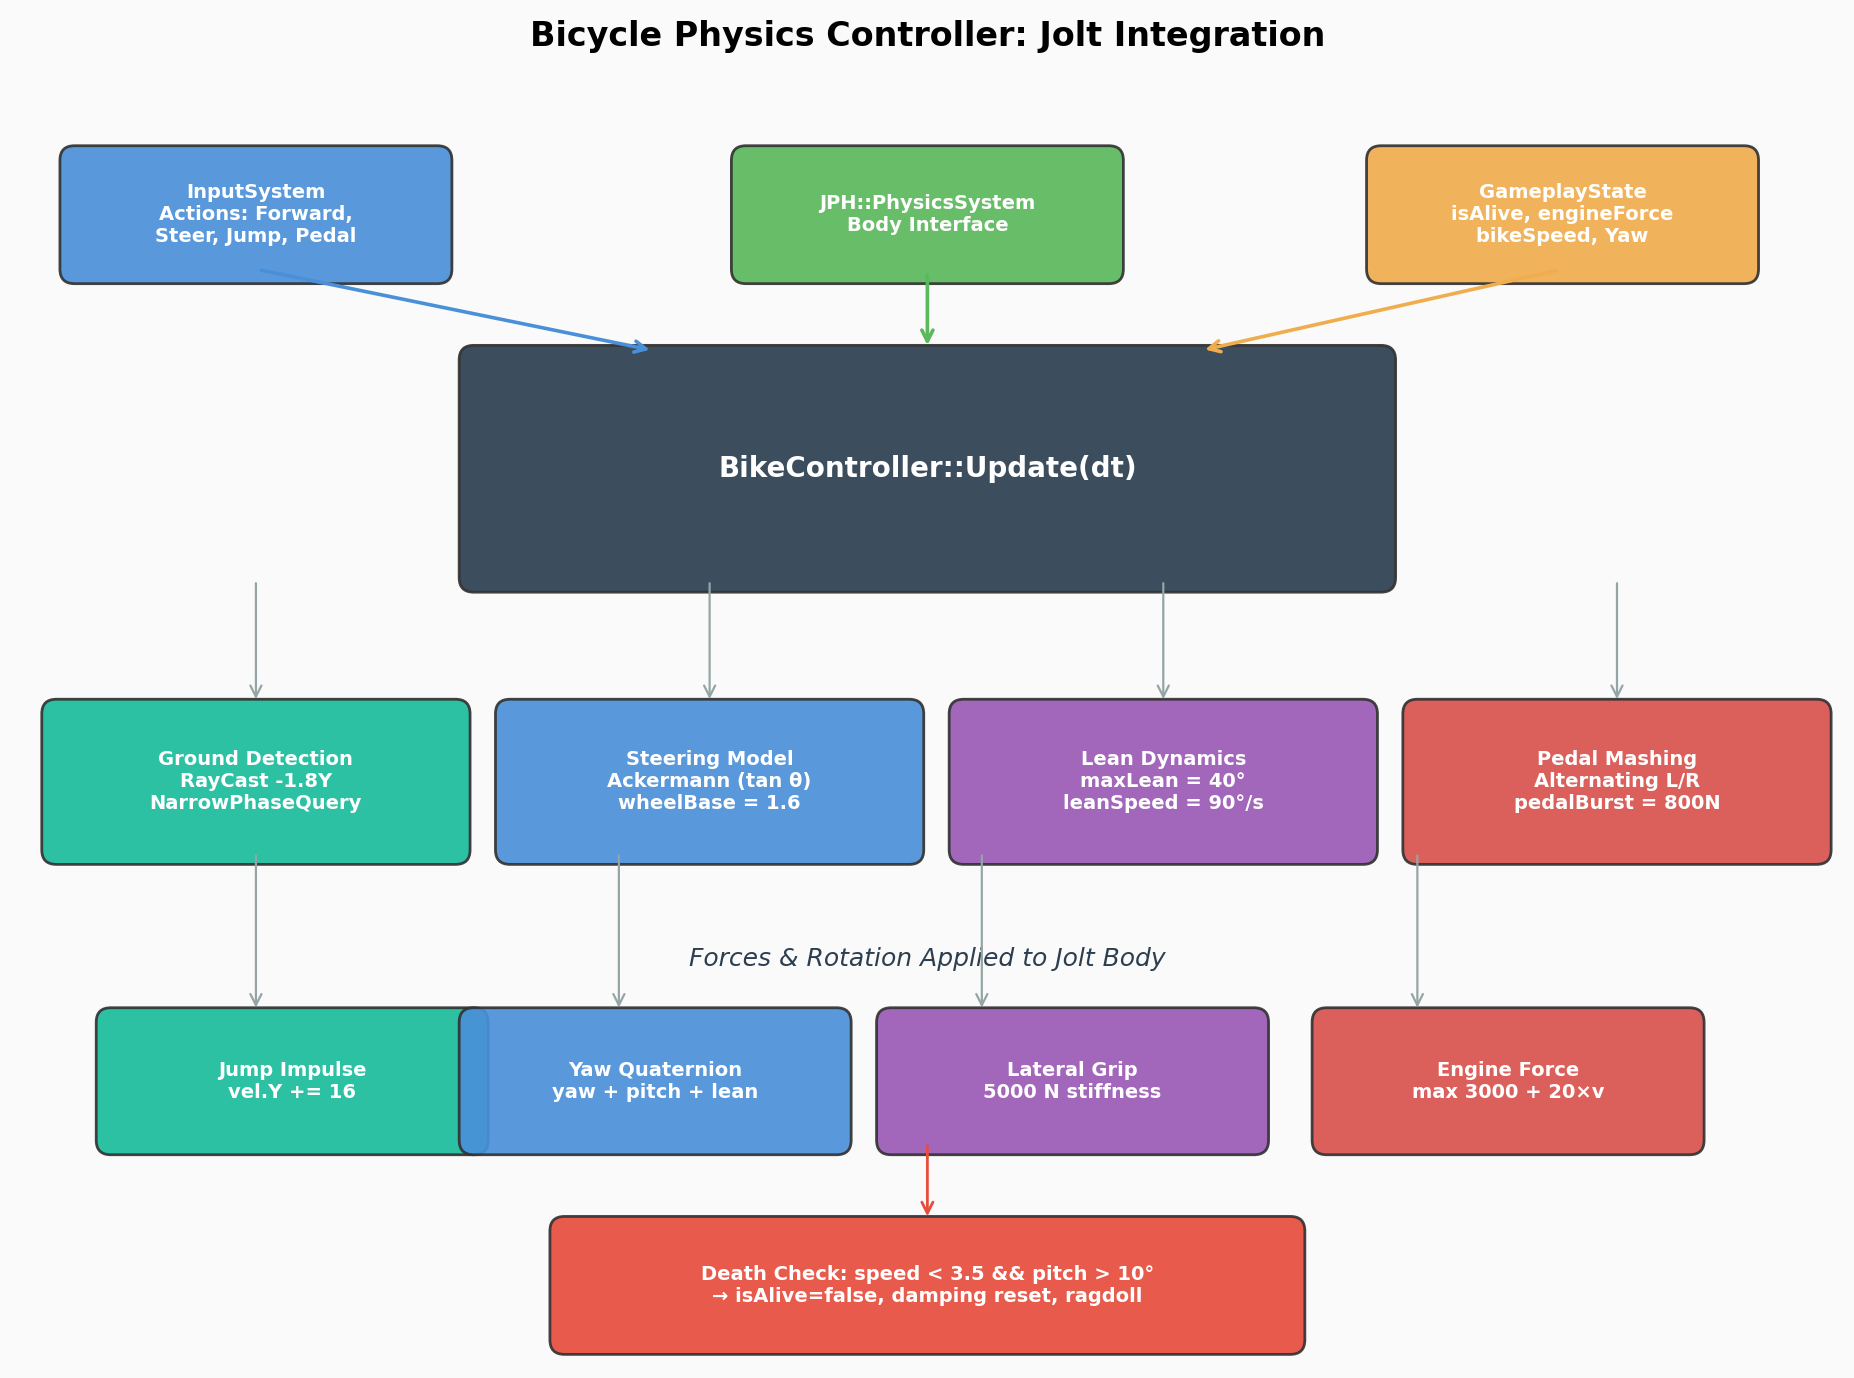
\includegraphics[width=\linewidth]{figures/vehicle_constraint_setup.png}
  \caption{\textbf{Vehicle Constraint Node Setup.} The Jolt \texttt{VehicleConstraint} hierarchy showing the chassis body, the two raycast wheel anchors, suspension spring parameters, and the user-data link back to the Flecs entity graph. Arrows indicate the per-tick data flow: input torques flow in, simulated transforms flow out.}
  \label{fig:vehicle_constraint}
\end{figure}
Consequently, when Jolt's collision listener fires a contact callback, we retrieve this payload, cast it back to a Flecs entity, and dispatch an engine-wide \texttt{CollisionEvent}. This elegantly bridges the object-oriented Jolt solver with our data-oriented Flecs architecture.

\subsection{Supporting Systems}

\subsubsection{Input System and Action Mapping}
To support a polished user experience, our \texttt{InputSystem} abstracts hardware-specific APIs into semantic gameplay actions. Rather than hardcoding \texttt{if (glfwGetKey(GLFW\_KEY\_W))}, systems poll an \texttt{ActionMap} for conceptual triggers like "Accelerate" or "Steer." 

The \texttt{InputSystem} hooks directly into GLFW's callback functions. For keyboard and mouse inputs, raw GLFW key codes are translated and stored in an internal state array, tracking whether a key is "Pressed," "Held," or "Released" during the current frame. This state is then evaluated against a user-defined configuration file that maps physical inputs to the abstract Action names. 

A significant challenge arose when implementing gamepad support, specifically mapping Xbox controllers within our Linux development environment via the \texttt{glfwGetJoystickAxes} API. Raw analog stick inputs are notoriously noisy, frequently registering minute values even when physically at rest, which previously caused our bicycle to drift endlessly. To mitigate this, we implemented a radial dead-zone filter. Given a raw 2D stick vector $\mathbf{s}$ and a dead-zone radius $d$ (typically 0.15), inputs with magnitude $\|\mathbf{s}\| \leq d$ are clamped to zero; inputs beyond the threshold are re-normalised so that the usable range $[d,\,1]$ maps linearly onto $[0,\,1]$, producing a smooth, drift-free response curve. A separate, smaller threshold ($d_{\text{cam}} = 0.1$) is applied independently to the right-stick camera-look axis to maintain responsive free-look without inadvertent yaw drift. This ensures precise, drift-free control over the \texttt{bikeController}'s steering constraints.

\subsubsection{Event System and the Observer Pattern}
Inter-system communication within a monolithic engine often leads to dangerous circular dependencies. To guarantee decoupled architecture, we implemented a robust Event System utilizing a C++ implementation of the Observer pattern.

Immediate dispatch could disrupt the memory state if an event triggers an entity deletion mid-iteration. To prevent this, we utilize a thread-safe \textbf{Event Queue} instead. When the \texttt{PhysicsSystem} detects a booster collision, it does not immediately call a function in the \texttt{SceneManager}. Instead, it allocates a \texttt{CollisionEvent} object and pushes it onto the back of the queue.

The \texttt{EventSystem} maintains a type-indexed subscriber map. Systems register callback functions keyed by \texttt{EventType} during engine initialisation. Rather than dispatching events immediately, events are enqueued into a thread-safe FIFO buffer protected by a mutex. This prevents the iterator state from being corrupted if a handler mutates the Flecs world mid-query. During the dedicated ``Event Processing'' phase of the main loop, the dispatcher drains the queue and broadcasts each event to all registered subscribers in registration order. If a subscriber marks the event as ``handled'', propagation halts, implementing a priority-based consumption model.

Systems register themselves as listeners during the \texttt{Application} initialization phase by binding function pointers (using \texttt{std::bind} or lambda expressions) to specific event types via a central \texttt{EventDispatcher}. During the designated "Event Processing" phase of our main game loop, the dispatcher iterates over the queue, broadcasting each event to all registered listeners simultaneously. This deferred execution ensures that circular dependencies are impossible: the physics system does not need to \texttt{\#include "SceneManager.hpp"}, it merely broadcasts that an event occurred into the void, allowing the Scene Manager to listen and react entirely independently.

\subsubsection{UI System and Vulkan Injection}
A modern engine requires robust, real-time developer tooling. We integrated the widely-adopted Dear ImGui library \cite{ImGui} created by Omar Cornut to handle all User Interface requirements.

Because our Vulkan rendering pipeline is strictly controlled via dynamic rendering passes, injecting the UI required meticulous orchestration. The \texttt{UISystem} operates as the absolute final sub-pass of the \texttt{RenderTick}. After the Main Forward pass and the Alpha-Masked pass have completed, we initiate a final \texttt{VkRenderingInfo} pass specifically targeted at the swapchain image. We pass the active Vulkan command buffer directly to \texttt{ImGui\_ImplVulkan\_RenderDrawData}, overlaying the UI graphics on top of the 3D scene immediately before the \texttt{vkQueueSubmit} call.

This immediate-mode GUI proved invaluable for debugging. Our custom debug windows tap directly into the engine's core metrics, exposing:
\begin{itemize}
    \item \textbf{Frametimes}: Tracking CPU logic ticks versus GPU render latency in milliseconds.
    \item \textbf{Draw Calls}: Displaying the exact number of \texttt{vkCmdDrawIndexed} submissions per frame, allowing us to actively verify that Frustum Culling is working correctly.
    \item \textbf{Physics Tuning}: Real-time sliders linked directly to the Jolt \texttt{VehicleConstraint} parameters, enabling us to tweak suspension stiffness and friction curves without recompiling the C++ codebase.
\end{itemize}

\subsubsection{Audio System (Miniaudio)}
To provide immersive auditory feedback without overwhelming the CPU, we implemented a dedicated \texttt{AudioSystem} leveraging the \texttt{miniaudio} single-header library. Miniaudio was selected for its minimal footprint and lack of external dependencies, directly aligning with our performance-focused ethos. The system provides an abstraction layer capable of parsing generic sound files and managing spatial/one-shot playback. Sound states (such as base volume, pitch, and runtime volume multipliers) are managed per-sound within a global hash map, ensuring rapid localized lookups during runtime events (such as booster collection or engine revving).

\subsubsection{Skeletal Animation and Inverse Kinematics (IK)}
While early development utilized static meshes, our engine now supports full Skeletal Animation evaluation. The \texttt{AnimationSystem} reads keyframe samplers and translates bone transformations. To dynamically integrate the player character with the vehicular simulation, we implemented a 2-bone Inverse Kinematics (IK) solver. The \texttt{RiderIKComponent} is attached to the character entity, defining specific chains (e.g., shoulder-elbow-hand). During the \texttt{AnimationSystem} update tick, the solver actively computes joint rotations to ensure the rider's hands remain firmly attached to the bicycle's handlebars, dynamically adapting to the bicycle's \texttt{LocalTransform} and steering vectors.

\subsubsection{Particle System Integration}
Visual feedback is essential for game feel, particularly during high-speed actions. We implemented a custom \texttt{ParticleSystem} supporting GPU-instanced rendering to minimize draw calls. Particles are emitted via configurable shapes (Cone, Sphere, Box) using randomized seed values to calculate unique lifetime, scale, and velocity vectors per particle. Memory allocations for particle pools are explicitly managed through Vulkan bindings via \texttt{volk}, allowing the engine to spawn thousands of dynamic particles (e.g., booster explosions or tire smoke) with negligible performance degradation.

Each particle is initialised with randomised lifetime, scale, and speed values drawn uniformly from artist-configurable $[\min, \max]$ ranges using independent $\mathcal{U}(0,1)$ samples. The initial velocity direction depends on the emitter shape: cone emitters perturb the up-axis by a spread angle $\sigma$, while sphere and box emitters apply analogous shape-specific sampling strategies. This randomisation ensures visually varied, non-repetitive particle clouds from a single emitter definition.

\subsubsection{Asset Upload Pipeline}
Modern Vulkan rendering strictly forbids the GPU from directly reading vertex and index data from system RAM if performance is a priority. To achieve optimal draw call performance, our engine implements a dedicated Asset Upload Pipeline utilizing Vulkan Staging Buffers.

When the \texttt{SceneManager} parses a level, the raw vertex and index data is initially loaded into system memory. We first allocate a temporary staging buffer using the \texttt{VK\_MEMORY\_PROPERTY\_HOST\_VISIBLE\_BIT | VK\_MEMORY\_PROPERTY\_HOST\_COHERENT\_BIT} flags. This allows the CPU to use \texttt{vmaMapMemory} to directly \texttt{memcpy} the raw geometry data into the buffer. 

However, this memory is slow for the GPU to read during rendering. Therefore, we allocate the final destination buffer on the GPU explicitly using the \texttt{VK\_MEMORY\_PROPERTY\_DEVICE\_LOCAL\_BIT} flag, which represents the fastest VRAM available. We then record a one-time-submit command buffer to execute a \texttt{vkCmdCopyBuffer} command:

The upload follows a three-stage process: (1)~allocate a host-visible staging buffer flagged for sequential CPU writes, (2)~map, copy, and unmap the raw data into the staging buffer, and (3)~record a one-time-submit command buffer containing a buffer-to-image (or buffer-to-buffer) copy targeting a device-local allocation. A fence synchronizes CPU-side cleanup: once the GPU signals transfer completion, the staging buffer is immediately destroyed, leaving geometry and texture data residing exclusively in the fastest available VRAM.

\begin{figure}[h]
  \centering
  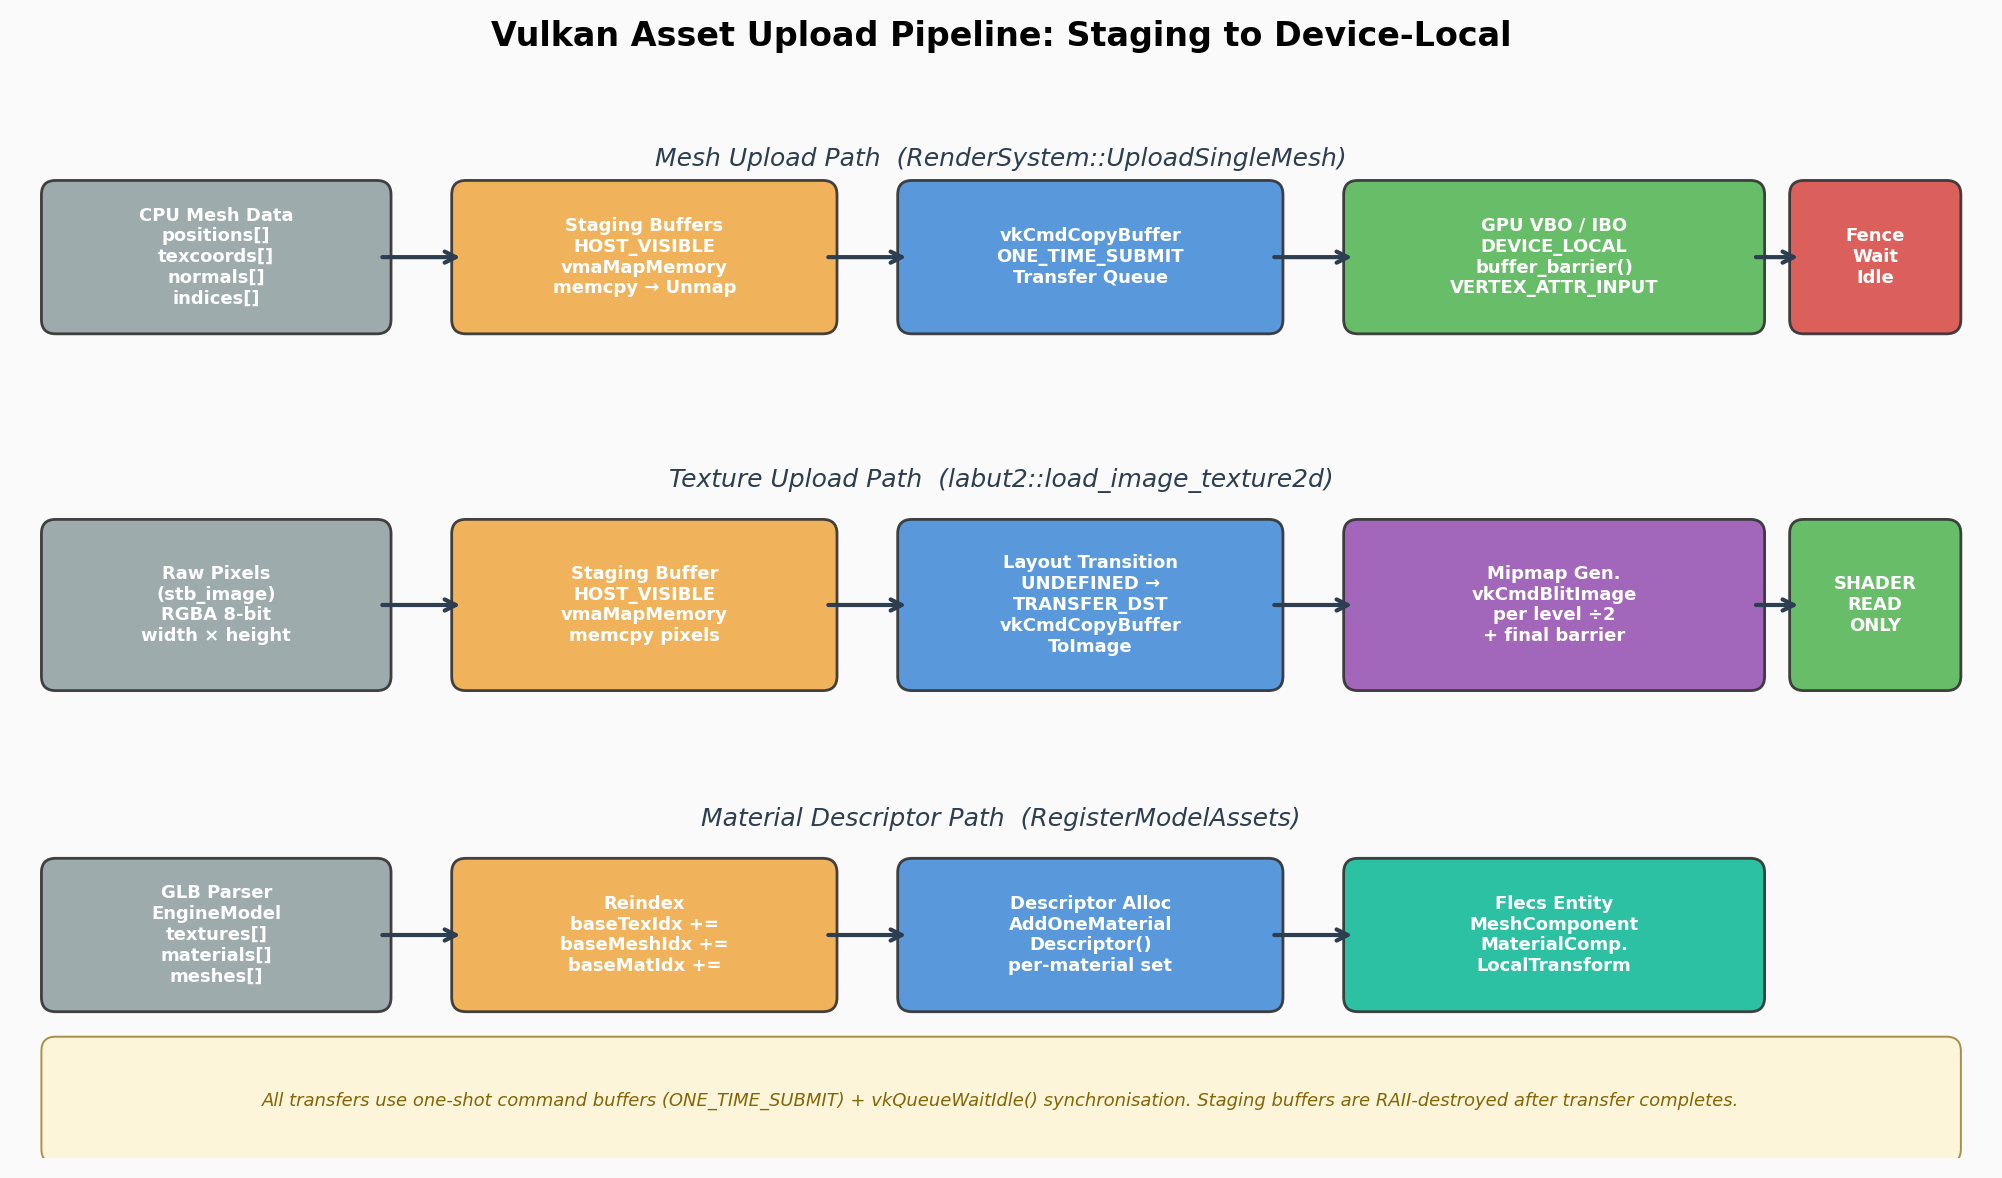
\includegraphics[width=\linewidth]{figures/asset_upload_pipeline.png}
  \caption{\textbf{Vulkan Asset Upload Pipeline.} Data flows from the \texttt{SceneManager} parser through a host-visible staging buffer, across a one-shot transfer command, and into device-local GPU memory. The fence-guarded handoff ensures the staging allocation is released immediately after the transfer completes.}
  \label{fig:asset_upload}
\end{figure}

After the transfer command is submitted and the GPU signals a fence upon completion, the CPU safely destroys the temporary staging buffer. This ensures that during the \texttt{Main Forward Pass}, the vertex shaders are pulling geometry exclusively from ultra-fast, dedicated GPU memory, entirely eliminating PCIe bus bottlenecks during the render loop.

\subsection{Implementation: The Biker Demo}
The bicycle action game serves as the primary technical demonstration of our engine's capabilities. The game loop emphasizes the synergy between the ECS logic, the vehicle physics, and the trigger mechanisms.

\subsubsection{Level Assembly Pipeline \& Geometry}
The level is assembled via the \texttt{SceneManager}, which orchestrates the loading of static objects (the ground, enclosing walls, and the ramp) and dynamic entities (the bicycle, the player, and collectible boosters). The level assembly pipeline parses custom scene formats and dynamically spawns Flecs entities, assigning rendering and collision components on the fly. 

The environment uses alpha-masked textures for fencing to demonstrate the multi-pass shadow pipeline, ensuring the lighting remains grounded and realistic even with complex overlapping geometry.

\subsubsection{Game Logic and the Biker Controller}
The player operates a physically simulated bicycle using input actions bound to acceleration and steering. To make the bicycle feel responsive, the \texttt{bikeController} dynamically manipulates the \texttt{VehicleConstraint} based on user input.

\textbf{Torque Application and Steering Vectors}: When the player presses the ``Accelerate'' input, we do not simply set a linear velocity. Instead, we apply a rotational torque to the rear wheel of the \texttt{VehicleConstraint}, calculated along the chassis forward vector $\hat{\mathbf{d}} = (-\sin\psi,\,0,\,-\cos\psi)$ derived from the current yaw $\psi$. The engine force $F_{\text{eng}}$ follows a burst--decay model: each pedal input increases the force by a burst impulse $F_{\text{burst}}$ scaled by a slope penalty $\kappa_{\text{slope}}$, clamped to $F_{\max}$; upon release, the force decays linearly at rate $r_{\text{decay}}$. To prevent unrealistic lateral sliding, a corrective grip force $\mathbf{F}_{\text{lateral}} = -v_{\text{lat}} \cdot k_{\text{grip}} \cdot \hat{\mathbf{r}}$ is applied along the chassis right-vector, where $v_{\text{lat}}$ is the lateral velocity component and $k_{\text{grip}}$ is a tunable coefficient. This allows controlled drifts at high speed while maintaining stable low-speed handling.

Steering modifies the angular limit of the front wheel. We map the horizontal analog stick input (ranging from -1.0 to 1.0) directly to a steering angle clamp (e.g., $\pm 30$ degrees). Jolt's constraint solver then automatically resolves the angular velocity, translating the forward torque into an arced trajectory.

\textbf{Suspension and Slope Adaptation}: The raycast suspension serves as the bicycle's shock absorbers. We configured the suspension's rest length and spring stiffness so that the rigid body floats slightly above the physical wheel ray hit points. This absorbs the immense vertical forces generated when landing from the jump ramp, preventing the chassis from flipping uncontrollably upon impact. To resolve initial collision bugs where the bicycle physics body clipped into terrain slopes, we implemented a robust pitch-adaptation system. Using raycasts, we actively align the bike's orientation with the underlying terrain slope, allowing the physics engine to properly resolve collisions for all parts of the chassis and preventing it from becoming embedded in ramps.

Friction was heavily tuned. Out-of-the-box rigid-body friction feels sluggish for a vehicle. We manually implemented a longitudinal vs. lateral friction curve constraint. As longitudinal velocity increases, lateral grip is artificially reduced, allowing the player to initiate controlled slides around tight corners, creating a nimble, arcade-like game feel, taking cues from the responsive handling of \textit{DiRT Rally} \cite{DirtRally} and \textit{Forza Horizon 5} \cite{ForzaHorizon5, ForzaPhysics}.

\subsubsection{Trigger Mechanisms \& Win/Fail Logic}
The central gameplay loop revolves around a collection mechanic.
\begin{itemize}
    \item \textbf{Boosters}: Scattered throughout the level are booster entities equipped with Trigger volume colliders. When the bicycle intersects a booster, the \texttt{PhysicsSystem} dispatches an overlap event. The event handler subsequently flags the booster for deletion. To prevent fatal table lock crashes when mutating Flecs entities mid-iteration (e.g., removing \texttt{PhysicsBody} components while the system is iterating), we utilized Flecs' deferred operations (\texttt{defer\_begin()} and \texttt{defer\_end()}). This ensures component structural changes are safely queued and executed at the end of the frame.
    \item \textbf{Level Completion \& Death Condition}: Once all boosters are collected, the user's state transitions to "Boost Mode", temporarily augmenting the bicycle's maximum torque and decreasing air-resistance logic. This enables the player to ascend the jump ramp at maximum velocity. We have also implemented a robust death condition loop; if the player fails to clear the ramp and crashes off the bike, the game detects the collision failure and triggers the death sequence, seamlessly resetting the level and preventing the player from phasing through boundaries or entering a soft-lock.
    \item \textbf{Win Condition}: A massive, invisible trigger volume is positioned just outside the enclosing walls. Successfully clearing the wall using the ramp causes the bicycle to intersect this volume, firing the "Level Complete" event. This immediately unloads the current Flecs component space and initializes the subsequent scene via the \texttt{SceneManager}.
\end{itemize}

\subsubsection{Camera System Architecture}
To effectively showcase the high-speed bicycle mechanics, we implemented a dynamic third-person camera that smoothly tracks the player without causing motion sickness. Simply locking the camera's position and rotation strictly to the Jolt \texttt{VehicleConstraint} rigid body results in an erratic, unplayable experience, as the bicycle's chassis violently pitches and rolls over uneven terrain.

To solve this, our camera operates as an independent Flecs entity that tracks a target position slightly behind and above the player's \texttt{WorldTransform}. We utilize a custom spring-damper mathematical model to interpolate the camera's current position towards the target position every frame.

For rotation, we completely decouple the camera's pitch and roll from the bicycle's physics. We instead calculate a "LookAt" matrix. We extract the bicycle's current translation vector and project a focal point slightly ahead of the front wheel. The camera then calculates a normalized direction vector pointing from its spring-damped position to this focal point:

The camera position $\mathbf{p}_{\text{cam}}$ is computed in spherical coordinates relative to a target point $\mathbf{t}$ offset above the player, parameterised by orbital distance $d$, yaw $\theta$, and pitch $\phi$. Each parameter is smoothed per frame via an exponential spring-damper with stiffness $s = 6.0$, interpolating towards the target orbit as $\theta(t + \Delta t) = \theta(t) + (\theta_{\text{target}} - \theta(t)) \cdot s \cdot \Delta t$, and analogously for $\phi$ and $d$. The final view matrix is constructed via $\text{lookAt}(\mathbf{p}_{\text{cam}},\,\mathbf{t},\,\hat{\mathbf{u}}_{\text{dyn}})$. This spring-damped orbit ensures the player remains comfortably centered in the frame, while the physical bicycle is allowed to dynamically bounce and bank independently beneath the focal point.

\section{Evaluation}
\textcolor{blue}{This section should cover how your project was evaluated. 
Regardless of the goal you are trying to achieve, a well designed evaluation should be considered. 
This section should describe what are the components you are trying to evaluate, and how the tests executed were the right ones for the purpose. 
This should be separated from considerations, as you might need to run several separate evaluations, and report distinct set of results that should be considered together. 
Use tables and graphs to communicate your results in an aggregated way, presenting the necessary information for the reader to comprehend your results quickly. 
While you could provide extra data in appendix, all that is necessary for comprehension of your results should be in the body of the report. 
Anyone reviewing your submission should not need to look at appendix to understand a core part of your manuscript. 
The appendix is not a workaround to the page limit, it is a bonus for really interested people. 
A good rule of thumb is: if my appendix is deleted, my report should still be comprehensible. 
}

To rigorously assess the technical soundness of our custom engine, we established specific testing methodologies targeting rendering efficiency, OS-level driver overhead, and hardware scaling. 

\subsection{Testing Environment \& Hardware Specifications}
Our benchmarking was conducted across two distinct hardware profiles to evaluate both architectural scaling and operating system overhead. 

\textbf{System 1: OMEN15 Laptop (Dual-Boot)}
\begin{itemize}
    \item \textbf{CPU:} AMD Ryzen 7 4800H (16 threads)
    \item \textbf{GPU:} NVIDIA GeForce GTX 1660 Ti
    \item \textbf{RAM:} 16.0 GiB (3200MT/s)
    \item \textbf{OS 1 (Linux):} Ubuntu 24.04.4 LTS (Kernel 6.17.0-23-generic)
    \item \textbf{OS 2 (Windows):} Windows 11 Home Build 26200
\end{itemize}

\textbf{System 2: UNI Lab PC}
\begin{itemize}
    \item \textbf{CPU:} 12th Gen Intel Core i7-12700 (20 threads)
    \item \textbf{GPU:} NVIDIA GeForce RTX 4070
    \item \textbf{RAM:} 30 GiB
    \item \textbf{OS:} Red Hat Enterprise Linux 9.7
\end{itemize}

\subsection{Methodology}
We performed a deterministic, automated camera fly-through of our heaviest scene geometry to ensure identical workloads across all tests. We focused on measuring Average FPS under two primary conditions: Frustum Culling Enabled vs Disabled. 
\begin{itemize}
    \item \textbf{OS Comparison (OMEN15):} To evaluate the Vulkan API's driver implementation differences, we ran identical Linux and Windows binaries on the exact same OMEN15 hardware. We utilized MangoHud for Linux telemetry and CapFrameX for Windows telemetry.
    \item \textbf{Hardware Scaling (Linux):} To test the engine's ability to utilize high-end hardware, we compared the mid-range GTX 1660 Ti against the high-end RTX 4070, executing the same Linux binary.
\end{itemize}

\subsection{Results: Frustum Culling \& OS Comparison}
The OMEN15 dual-boot testing yielded clear performance data regarding both our engine optimizations and the underlying Vulkan drivers. 

\begin{figure}[h]
  \centering
  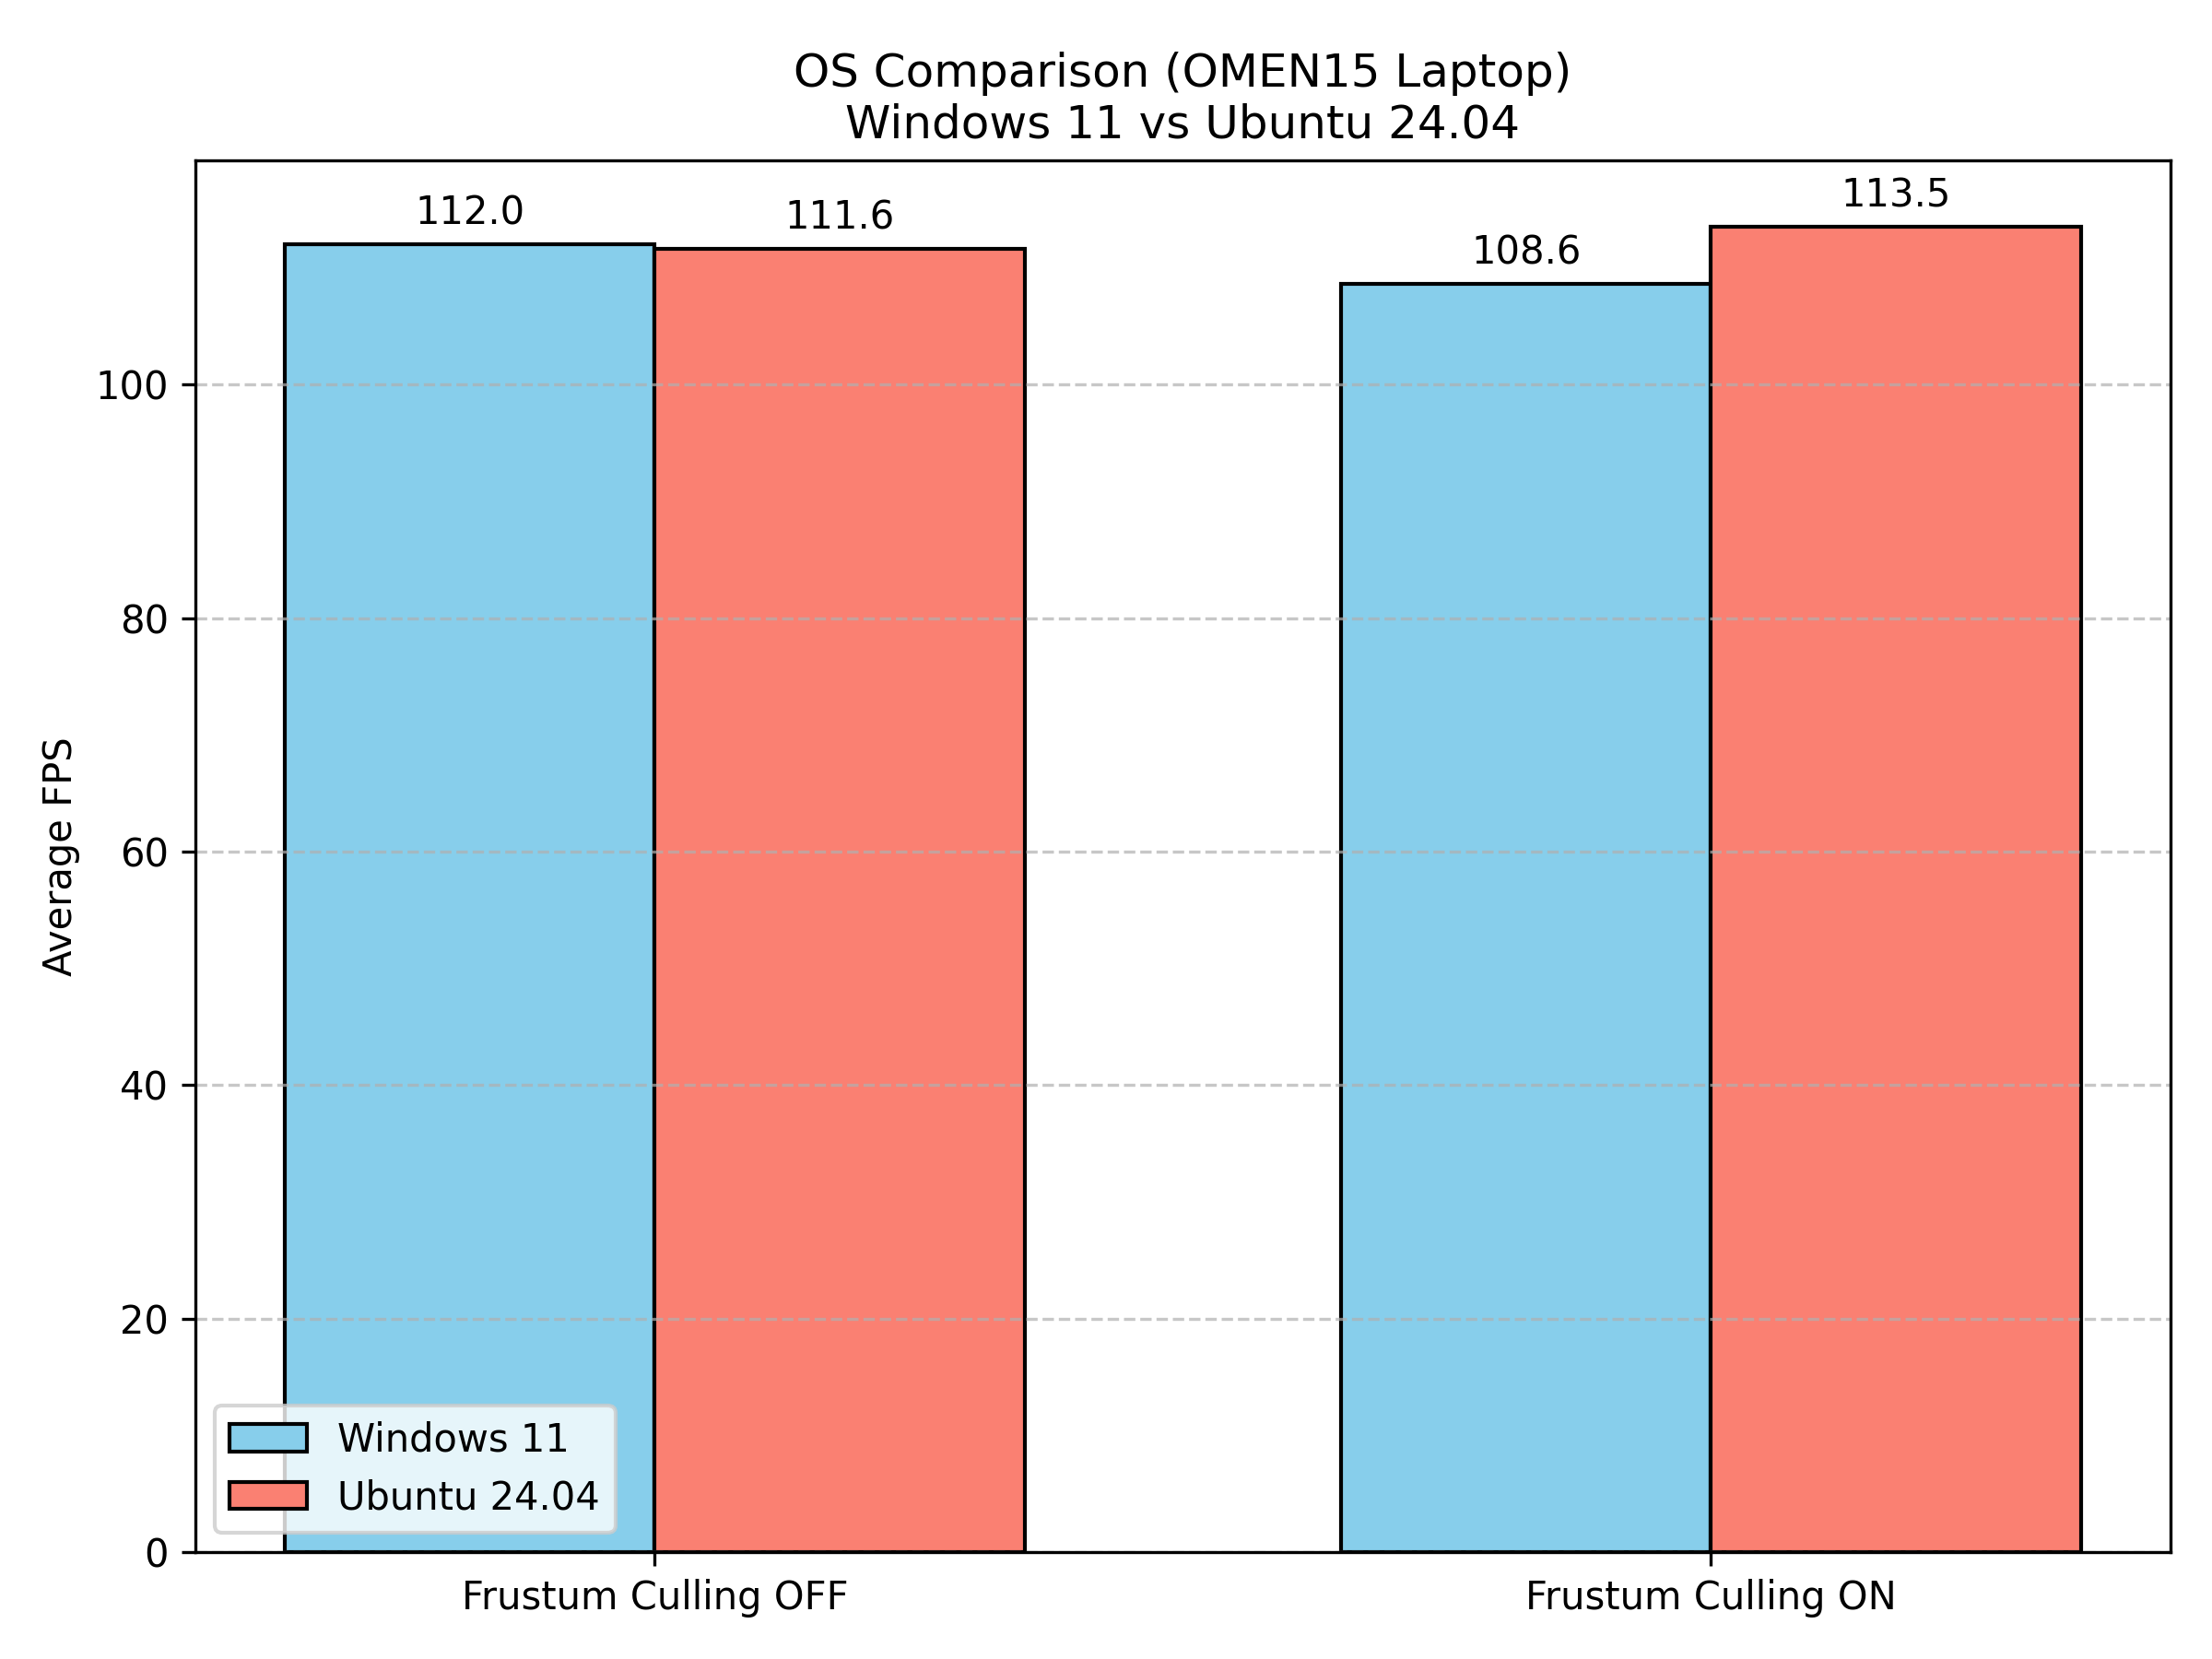
\includegraphics[width=\linewidth]{figures/Chart1_OS_Comparison.png}
  \caption{\textbf{OS Comparison.} Average FPS on identical OMEN15 hardware (GTX 1660 Ti) comparing Windows 11 and Ubuntu 24.04.}
  \label{fig:os_comparison}
\end{figure}

Ubuntu 24.04 performed slightly worse than Windows 11 with culling off ($111.6$ FPS vs $112.0$ FPS), but significantly outperformed Windows 11 when culling was enabled ($113.5$ FPS vs $108.6$ FPS). On Linux, enabling Frustum Culling improved the average framerate from $111.6$ FPS to $113.5$ FPS, confirming that our CPU-side culling successfully reduces Vulkan submission overhead. Conversely, the performance regression on Windows when Frustum Culling was enabled indicates potential differences in how the Windows NVIDIA Vulkan driver handles dynamic command buffer recording and CPU-side branching compared to the Linux driver.

\subsection{Results: Hardware Scaling}
The hardware scaling test evaluated how the engine performs on high-end desktop components versus mobile architectures.

\begin{figure}[h]
  \centering
  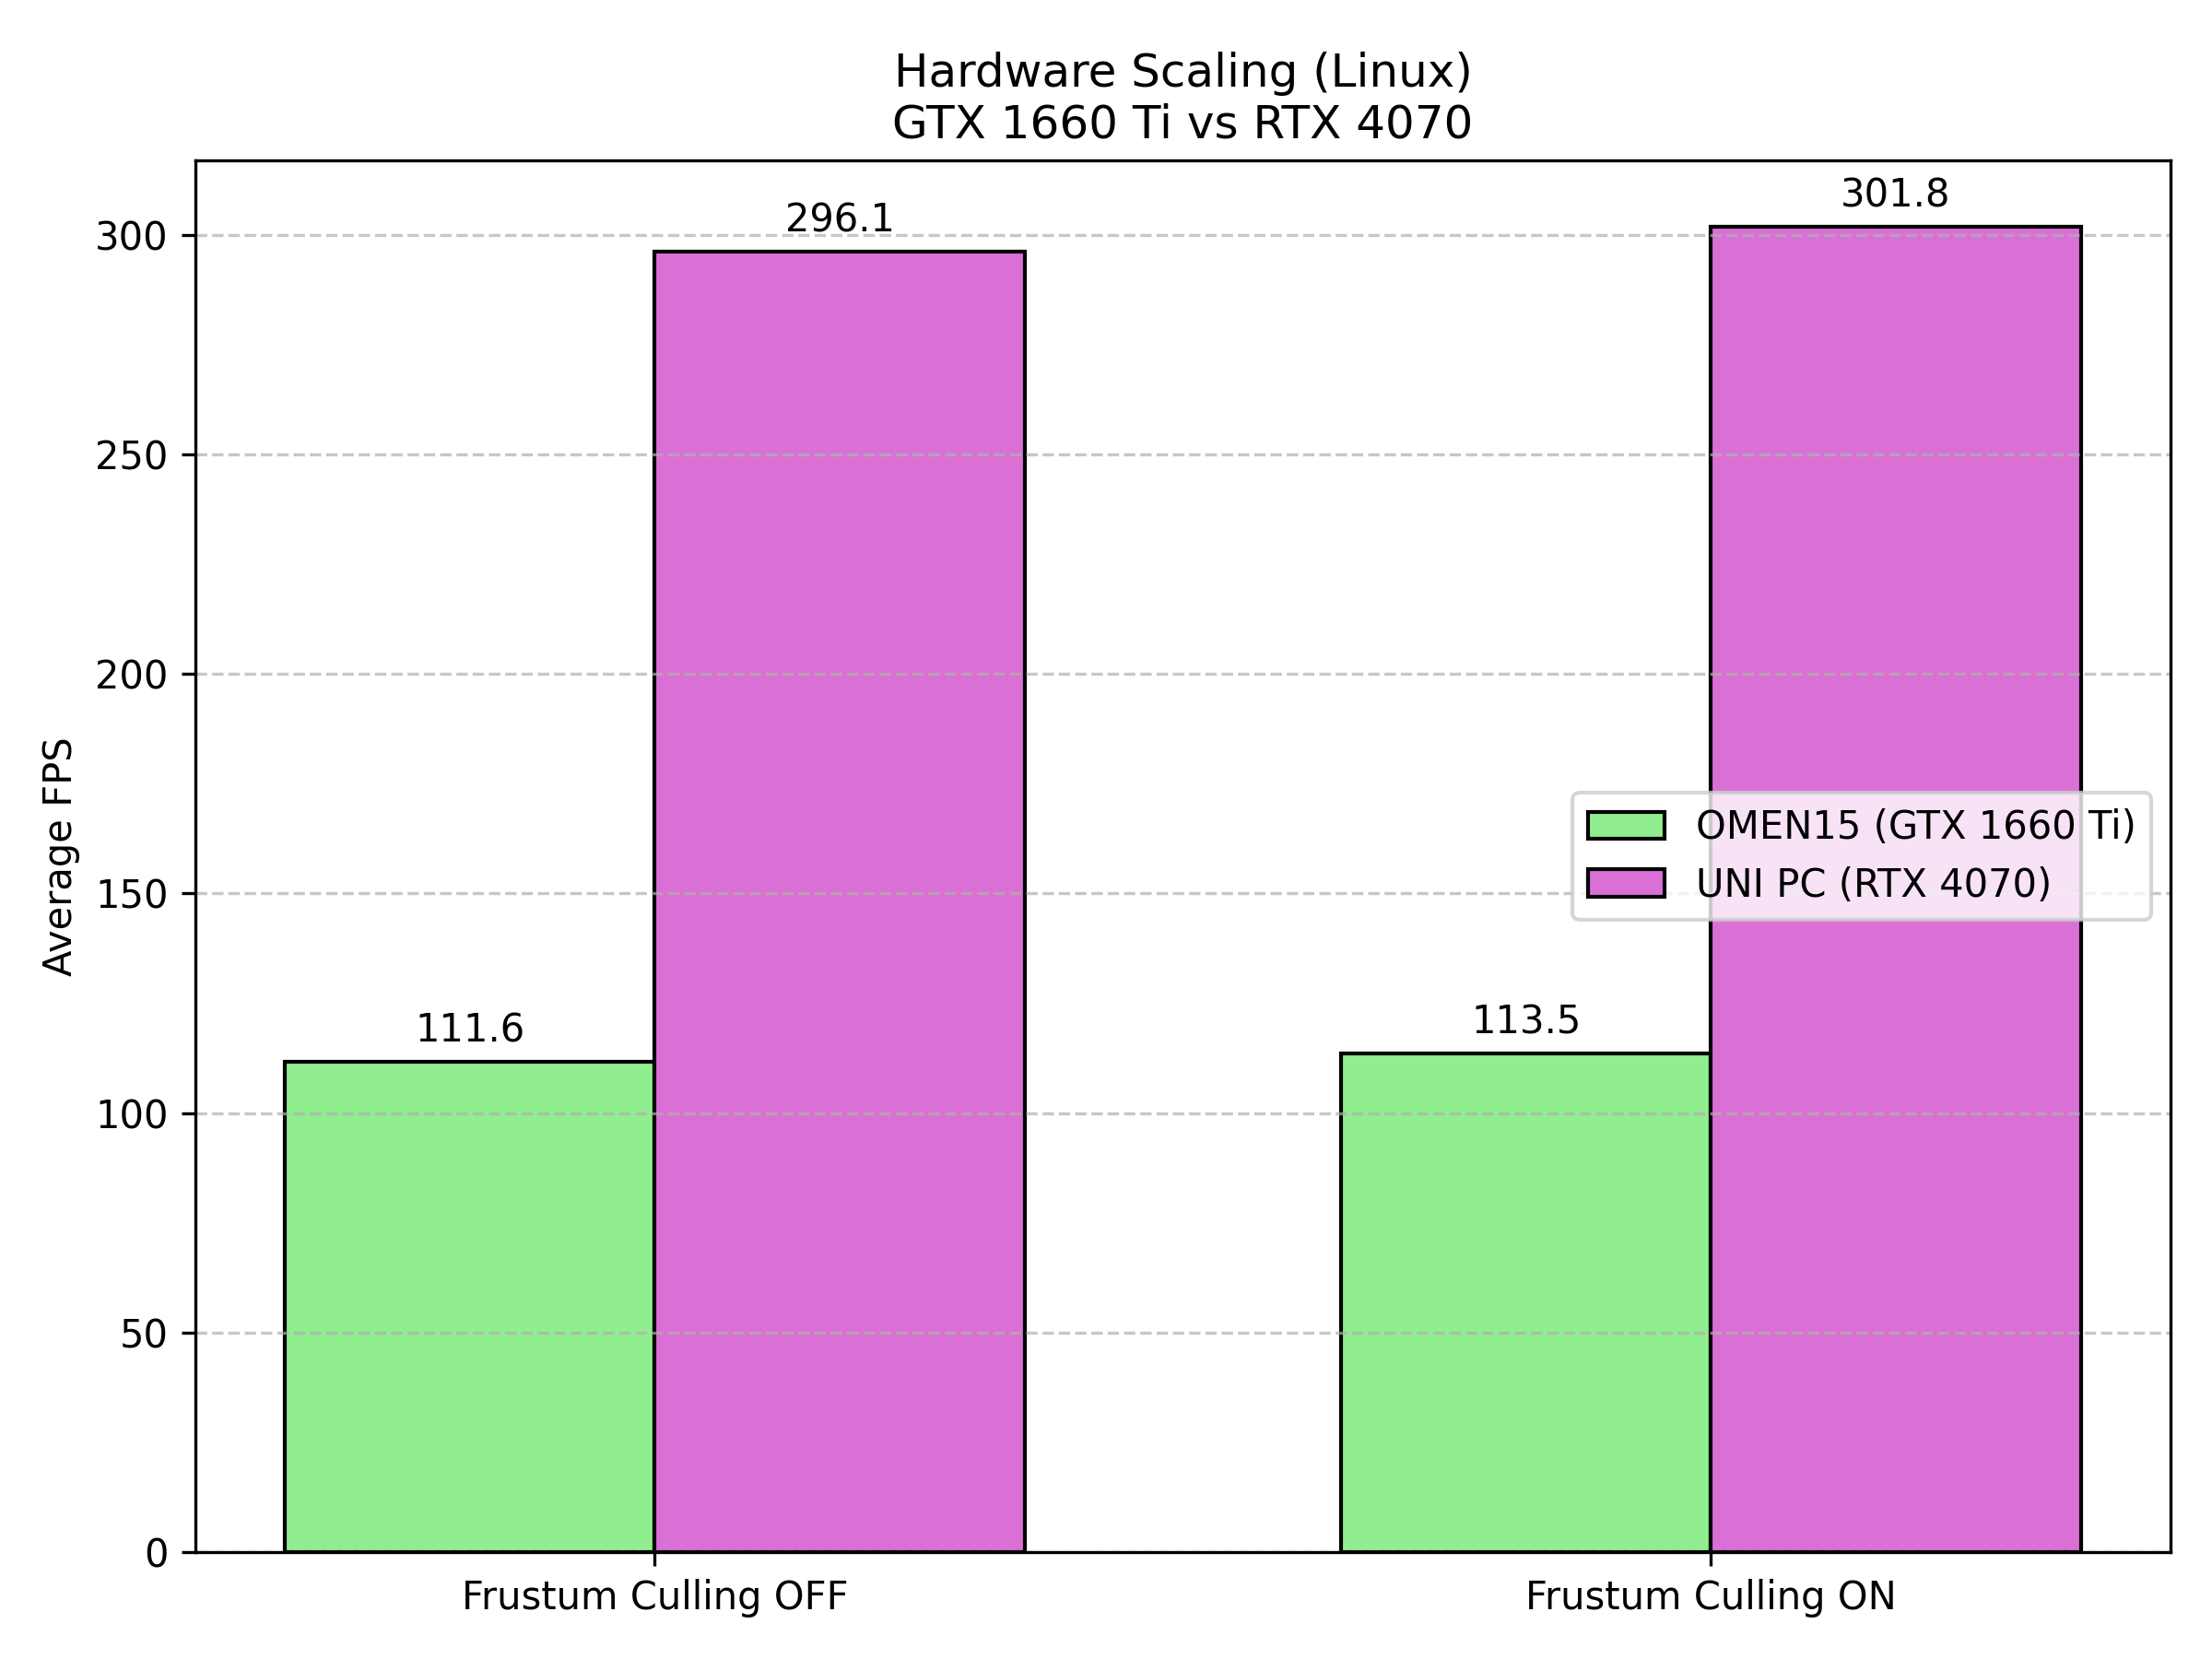
\includegraphics[width=\linewidth]{figures/Chart2_Hardware_Scaling.png}
  \caption{\textbf{Hardware Scaling.} Average FPS on Linux comparing the OMEN15 Laptop (GTX 1660 Ti) and the UNI Lab PC (RTX 4070).}
  \label{fig:hardware_scaling}
\end{figure}

While the OMEN15 produced $111.6$ FPS (Off) and $113.5$ FPS (On), the high-end UNI Lab PC (RTX 4070) initially delivered a locked $100.0$ FPS in both tests. This initial lock was traced back to the engine's default Vulkan presentation mode (\texttt{VK\_PRESENT\_MODE\_FIFO\_KHR}), which enforced V-Sync and artificially capped the framerate to the lab monitor's 100Hz refresh rate. To accurately measure the hardware limits, we explicitly modified the RHI layer to request an uncapped presentation mode (\texttt{VK\_PRESENT\_MODE\_IMMEDIATE\_KHR} or \texttt{VK\_PRESENT\_MODE\_MAILBOX\_KHR}).

With the V-Sync limit removed, the RTX 4070 demonstrated massive processing headroom, skyrocketing to $296.1$ FPS (Off) and $301.8$ FPS (On). This nearly 2.6x performance delta compared to the GTX 1660 Ti definitively proves that the engine's underlying architecture scales exceptionally well on high-end desktop hardware when not bottlenecked by synchronization limits.

\section{Discussion}
\textcolor{blue}{This is where you actually draw conclusions from your results, and discuss how successful or not things were. 
This is where we would like to see your critical analysis of the method and the results. 
Provide unique insights on why do you think you achieved the results you did in the previous section, do not limit yourself to stating the obvious.}

Building a custom Vulkan engine from the ground up to support a specialized vehicular game was an immensely challenging but rewarding endeavor. Rather than battling the generalized rigidity of an engine like Unreal, we were able to surgically optimize our collision detection and memory layout for exactly what we needed.

\textbf{Handling Feedback:}
One of the key improvements from earlier assignments was the overhaul of the shadow mapping system. We received critical feedback highlighting the lack of shadow hardware PCF (resulting in massive errors when scaling resolution) and the absence of \texttt{textureProj} lookups. We directly addressed this by entirely rewriting the shadow shader bindings, ensuring proper perspective division via \texttt{textureProj}, and binding \texttt{sampler2DShadow} to enable native GPU filtering. The results completely eliminated the aliasing artifacts.

\textbf{Engine Limitations:}
Our decision to use pure ECS (Flecs) came with a steep learning curve. While it eliminated OOP-related spaghetti code, debugging state mutations required building custom ImGui visualisations, as standard debugger step-throughs were often unhelpful inside generic system iterators.

Additionally, the initial challenges with gameplay integration for our Particle System have been resolved, allowing for synchronized visual effects (like booster explosions and tire smoke) directly tied to event triggers. Similarly, the successful integration of the Miniaudio \texttt{AudioSystem} significantly elevates the game feel, ensuring that collecting boosters and landing jumps are accompanied by impactful, low-latency auditory feedback.

\section{Conclusion}
\textcolor{blue}{Here you draw things to a close.
It should be a much shorter version of your introduction, without the motivation part, but focusing on your results, and what it leads to going forward. 
You can have clear sections for limitations and future work, or work it into the text of your conclusion.}

The Steer Engine successfully demonstrates that a targeted, performance-centric architecture can yield rapid, flexible development for specialized games. By marrying the data-locality of Flecs ECS with the raw performance of Vulkan and Jolt Physics, we established a pipeline capable of processing complex level geometry, PBR lighting, and robust vehicular dynamics.

Having successfully integrated full skeletal animation IK and a robust sound system, the demo game delivers a highly polished experience. The core loop proves the engine's capability to seamlessly handle event-driven gameplay logic, concurrent physics simulation, and dynamic audio-visual feedback simultaneously. This loop consists of traversing the level, collecting boosters, gaining speed, and clearing the ramp. The project succeeded in its primary goal: establishing a technical foundation that out-performs generalised architectures for this specific domain.

\begin{acks}
The group are thankful to the university staff and TAs for their guidance and feedback throughout the project.
\end{acks}

\begin{thebibliography}{99}

\bibitem{JoltHorizon} Jorrit Rouwe. 2021. Physics Animation in Horizon Forbidden West. GDC 2021.
\bibitem{HorizonFW} Guerrilla Games. 2022. Horizon Forbidden West. Sony Interactive Entertainment.
\bibitem{NFSUnbound} Criterion Games. 2022. Need for Speed Unbound. Electronic Arts.
\bibitem{NFSUnboundTech} Oliver Mackenzie. 2022. Need for Speed Unbound tech review. EuroGamer.
\bibitem{Flecs} Sander Mertens. 2025. Flecs: A fast and lightweight C/C++ ECS. https://github.com/SanderMertens/flecs
\bibitem{JoltPhysics} Jorrit Rouwe. 2025. Jolt Physics. https://github.com/jrouwe/JoltPhysics
\bibitem{VulkanSpec} Khronos. 2025. Vulkan Documentation.
\bibitem{ImGui} Omar Cornut. 2025. Dear Imgui.
\bibitem{GLFW} Marcus Geelnard. 2025. GLFW.
\bibitem{CookTorrance} R. L. Cook and K. E. Torrance. 1982. A Reflectance Model for Computer Graphics. ACM Transactions on Graphics.
\bibitem{Schlick} Christophe Schlick. 1994. An Inexpensive BRDF Model for Physically-Based Rendering. Computer Graphics Forum.
\bibitem{Beckmann} P. Beckmann and A. Spizzichino. 1963. The Scattering of Electromagnetic Waves from Rough Surfaces. Macmillan.
\bibitem{RocketLeague} Psyonix. 2015. Rocket League. Psyonix.
\bibitem{OverwatchECS} Timothy Ford. 2017. Overwatch Gameplay Architecture and Netcode. GDC 2017.
\bibitem{DestinyECS} Chris Tchou. 2017. Destiny's Multithreaded Rendering Architecture. GDC 2017.
\bibitem{DoomEternal} id Software. 2020. DOOM Eternal. Bethesda Softworks.
\bibitem{DoomVulkan} Axel Gneiting. 2016. The devil is in the details: idTech 6. SIGGRAPH 2016.
\bibitem{VMA} Adam Sawicki. 2025. Vulkan Memory Allocator. AMD GPUOpen.
\bibitem{DataOrientedDesign} Richard Fabian. 2018. Data-Oriented Design.
\bibitem{GameEngineArch} Jason Gregory. 2018. Game Engine Architecture, Third Edition. CRC Press.
\bibitem{BulletPhysics} Erwin Coumans. 2025. Bullet Real-Time Physics Simulation.
\bibitem{PhysX} NVIDIA. 2025. NVIDIA PhysX SDK 4.0.
\bibitem{CyberpunkVulkan} CD Projekt Red. 2020. Cyberpunk 2077. CD Projekt.
\bibitem{ForzaHorizon5} Playground Games. 2021. Forza Horizon 5. Xbox Game Studios.
\bibitem{ForzaPhysics} Chris Tector. 2014. Forza Motorsport 5: Next-Generation Physics. GDC 2014.
\bibitem{DirtRally} Codemasters. 2015. DiRT Rally. Codemasters.
\bibitem{MarioKart8} Nintendo EAD. 2014. Mario Kart 8. Nintendo.
\bibitem{OpenGLSuperBible} Graham Sellers. 2015. OpenGL SuperBible. Addison-Wesley.
\bibitem{RealTimeRendering} Tomas Akenine-Möller. 2018. Real-Time Rendering. A K Peters.
\bibitem{LearnVulkan} Alexander Overvoorde. 2025. Vulkan Tutorial.
\bibitem{GTA5} Rockstar North. 2013. Grand Theft Auto V. Rockstar Games.
\bibitem{Frostbite} Electronic Arts. 2025. Frostbite Engine Documentation.
\bibitem{Wipeout} Studio Liverpool. 2008. Wipeout HD. Sony Computer Entertainment.

\end{thebibliography}

\newpage
\appendix

\section{Project management}
\textcolor{blue}{This is the appendix of your report, which should contain all the project management details, distinct from the scientific content of it. 
Please follow this rough structure, including everything you deem necessary up to the page limit of 6.}

\subsection{Supervisor and Theme}
\textcolor{blue}{Write a short description of how the theme of the project and the supervisor were chosen.
Do not go into long narratives, but this should highlight the good match between the groups interests and the supervisors area of expertise.
Mention how often you had contact with your supervisor, and rough structure of these meetings. 
It should be clear what was their goal. }

Text

\subsection{Group organization}
\textcolor{blue}{What was the adopted development strategy?
How was the group organized? 
Did you have teams?
What are the chosen communication channels? 
How did you organize the code? 
Did you use version control? 
How often did you meet? 
What was the goal of the meetings? 
What measures you had in place to keep everyone in track?
What measures you had in place to ensure deadlines were met?
What measures you had in place to evenly distribute work?}

The group dynamic was generally very positive, though it naturally experienced the stress associated with impending deadlines. We established a shared technical vocabulary early on and communicated primarily through a shared Discord server, documenting our API contracts meticulously.

Work distribution was handled fairly and transparently based on individual strengths and interests. The labor was divided across major systems: the Vulkan Renderer Port and Shadow System, Jolt Physics Integration and vehicle control, Flecs ECS integration, and overarching Scene Management. Sometimes team members struggled with specific issues, such as mapping Linux Xbox controller inputs into the generic Input System. When this happened, those who had finished their tasks early stepped in to pair-program solutions. We utilized a strict Git branching strategy (\texttt{feature/} branches merging into main), preventing individual experiments from breaking the master build. Features deemed too complex for the timeframe, such as the Animation State Machine, were collectively agreed upon to be marked as 'in development' to prevent burnout.

\subsection{Planning and execution}
\textcolor{blue}{This should contain two gantt charts: the initial planning, and what actually ended up happening.
The text in this section should be a reflection of why there was any different between them, or a reflection on why it was the right choice of planning in case they are exactly the same. }

[in progress; not done yet]

At the beginning of the semester, our initial plan was highly structured. We allocated specific weeks for engine architecture, rendering milestones, physics integration, and gameplay scripting. However, we underestimated the cascading complexities that arise when porting individual assignments into a unified monolithic architecture managed by Flecs. Creating a pipeline that seamlessly translated raw level data into Flecs entities, Jolt physical bodies, and Vulkan render batches took nearly four weeks instead of the planned two. Because we front-loaded the most critical architectural tasks, the delays did not completely derail the project, and we retained a functioning core loop early enough to pivot our gameplay mechanics.

The most significant test of our adaptability occurred mid-semester during a major crisis regarding our game design. Our original concept was an atmosphere-heavy game set in a "Silo" featuring an "ICBM Trigger" and underground environments. It became clear that an enclosed environment actively fought the strengths of our engine, which excelled at high-speed vehicular dynamics and expansive outdoor lighting. Realising that the ICBM concept was disjointed from our technological achievements, we made the difficult but necessary decision to completely scrap the underground game and pivot to the current Bicycle Action Game. Because our engine was heavily decoupled via the ECS architecture, we didn't have to rewrite the rendering or physics cores. This agile response saved the project from becoming a technical mismatch.

\section{Self-reflection and soft skills acquired.}
\textcolor{blue}{Overall conclusion of the project from a management point of view. 
Besides the technological and scientific aspects of your project, what did you learn as a group, and how may that be useful in the workforce, hopefully soon? Please provide individual reflections from different group members. Group please make sure what they say is true.}

This project was a crucible for developing professional soft skills that go far beyond the taught material. First and foremost, we learned the critical importance of \textbf{Technical Negotiation}. When integrating different systems, we frequently had to negotiate API boundaries. Learning how to compromise and design components to satisfy both rendering and physics requirements without causing friction was a massive learning experience.

Secondly, we developed robust \textbf{Agile Adaptability}. Scrapping the ICBM game taught us not to succumb to the "sunk cost fallacy." In the real workforce, requirements change, and features get cut. Learning to emotionally detach from discarded code and pivot towards a more viable product is an invaluable skill.

Finally, we refined our \textbf{Cross-Disciplinary Communication}. Writing engine code requires explaining abstract memory management concepts to team members focused on level design. We learned how to write clear, concise documentation and how to give constructive code reviews that focused on logic and performance rather than personal coding styles.

\section{How ethical issues are addressed}
\textcolor{blue}{This is a University requirement. See Resources on 'Ethics relevant to computing projects' for guidance and discuss it with your supervisor. If no ethical issue is involved, a sentence to that effect will suffice.}

No specific ethical issues are involved in the scope of this generic game engine project.

\end{document}
\endinput
%%
%% End of file `main.tex'.
